%!TEX root = ../thesis.tex
% ******************************* Thesis Appendix A ****************************
\chapter{Supporting work for \autoref*{chap:clustering}}

% ===========================================================

\section{DNA sequencing methods}

\subsection{DNA extraction}

\subsubsection{Madagascar}

\todo[inline]{waiting to see if Simon or Niaina have changes or additions to this}

DNA from MTB culture was extracted using the cetyltrimethylammonium bromide (CTAB) method previously described by Van Embden with little modification (Van Embden et al., 1993). Briefly, Sample was inactivated by heating at 80 ° C for 30 minutes. Lysozyme 10 mg / ml is added to the suspension and sample is incubated for at least one hour at 37 ° C. After addition proteinase K 10 mg / ml and sodium dodecyl sulfate (SDS) 10\%, the suspension was incubated for 10 min at 65 ° C. Mixture of CTAB and 5M NaCl preheated to 65 ° C was the added. The suspension was mixed until a milky mixture was obtained and incubated for 10 minutes at 65ºC. Chloroform: isoamyl alcohol (24:1) mixture was added followed by centrifugation for 5 min at 10,000 rpm, + 4 °C. The upper phase was recovered and DNA was precipitated by adding isopropanol to the solution.  The mixture was frozen at least for one hour then centrifuged at 10000rpm at, + 4 ° C, for 5min.  The supernatant was discarded and pellet was washed with 70\% ethanol and centrifuged at 10,000 rpm, + 4 ° C, for 5 min. The DNA pellet was dried at speed-vac for 2min and resuspended in 1X TE. DNA was quantified using the Qubit dsDNA HS Assay Kit (Thermo Fisher Scientific, USA).

% Van Embden J, Cave MD, Crawford JT, Dale J, Eisenach K, Gicquel B, et al. Strain identification of Mycobacterium tuberculosis by DNA fingerprinting: recommendations for a standardized methodology. Journal of clinical microbiology. 1993;31(2):406-9.

\subsection{Illumina}

\towrite[inline]{once i get this info from collabs}

\subsection{\ont{}}

\towrite[inline]{once i get this info from collabs}

\subsection{PacBio}
\label{app:pacbio-seq}

35 of the Malagasy samples were sequenced and processed at the Next Generation Genomics Core within Cold Spring Harbor Laboratory. Samples were quantified with a Qubit dsDNA HS Assay Kit and QC’d through a Pulsed Field Gel Electrophoresis system. Then, samples were sheared at 10kb using a Megaruptor device and size-selected to 8-10 kb with a Blue pippin instrument - followed by 0.45X ampure bead purification. The PacBio library protocol SMRTbell Express Template Prep Kit 2.0 was used for each sample. Briefly, the first step was the removal of single-stranded overhangs followed by DNA Damage Repair, End-Repair/A-tailing, Ligation of overhang barcoded adaptors and sample pooling. A total of 3 pools were produced: LID50532 (16 samples), LID50533 (10 samples), and LID50534 (9 samples). After pooling, 0.5X ampure bead clean up was performed. A Sequel I instrument was used to sequence the 3 library pools. Libraries were annealed for an hour and bounded for an hour using sequel binding kit 3.0. Bound SMRTbell complexes were then purified with ampure beads. The run was set up as 10kb length for 10 hours movie time. The Sequel 1M V2 SMRT cells were used for each library.  

The circular consensus was called via the SMRTlink graphical user interface version 6.0.0.47841.

% ===========================================================

\section{Benchmark of long read genome assembly methods for \mtb{}}
\label{app:asm}
We chose samples with greater than 30x coverage across all three sequencing technologies to produce high-quality assemblies. In total, this left 9 Malagasy samples. There have been many new genome assembly methods produced since the last known assessment of \mtb{} long-read assemblies \cite{bainomugisa2018}. As such, we compare five assemblers and select the one that produces the most consistently good results. The reason for this comparison is that different assembly algorithms can produce quite varied results depending on sequencing technology used, species, or computational resource availability \cite{demaio2019,wick2020}.  

As outlined in \autoref{sec:asm_results}, the assembly tools we assess are Canu, Flye, Unicycler, HASLR, and Spades. \haslr{} and \unicycler{} are hybrid assemblers that take Illumina reads along with one long-read file. \spades{} is also a hybrid assembler but takes an arbitrary number of different sequencing technologies. \canu{} and \flye{} are both long-read-only assemblers.

The first step in the assembly pipeline is trimming adapter sequences in the Illumina reads using Trimmomatic (v0.39; \cite{bolger2014}). Two assemblies were produced for each sample - one for each long-read technology. The exception to this was \spades{}, for which there is just one assembly for each sample, as it accepts all reads simultaneously. 

\canu{}, in some cases, produces assembly bubbles, which are regions where it believes there is a heterozygous locus due to differences in haplotypes. While some samples could be multi-clonal, we chose to remove bubbles from the \canu{} assemblies, effectively choosing the dominant haplotype for downstream analysis.  

All contigs in the resulting assemblies were species-classified using Centrifuge (v1.0.4beta; \cite{kim2016}). We remove any contigs whose classification places them outside of the Mycobacterium Tuberculosis Complex. Polishing these decontaminated assemblies is done in two steps; first using long-reads and Racon (v1.4.13; \cite{vaser2017}) with default settings, followed by short reads with Pilon (v1.23; \cite{pilon2014}). Default Pilon settings were used for \ont{} assemblies, but for PacBio we do not correct for SNPs. PacBio CCS reads are already a consensus from multiple reads, so allowing Illumina reads to fix at a per-base level lead to decreased per-base accuracy (results not shown).  

We annotate both the polished and unpolished genome assemblies using Prokka (v1.14.5; \cite{seeman2014}). We assess the relative correctness of all assembly variations for a given sample using Assembly Likelihood Estimator (ALE; \cite{clark2013}). Assembly statistics were generated for each sample using Quast \cite{quast2013} with the \mtb{} reference genome, H37Rv (accession: NC\_000962.3), as a reference. We do not expect our assemblies to be the same as H37Rv, but it can provide insights into the structural completeness and genome size. Lastly, we assess per-base accuracy using a custom script. As input for the script, we provide a BAM file of the Illumina reads mapped to the assembly and the pileup generated by the Samtools subroutine \vrb{mpileup} \cite{samtools2009}. We require a quorum of 90\% and a minimum read depth of 10x. Quorum is the percentage of reads that must agree with the assembly at each position. Any position in the assembly that does not meet both of these conditions is considered a disagreement. The output from the script is a collection of statistics and a BED file containing all disagreement positions.

Assessing the quality of \denovo{} assemblies is non-trivial and requires aggregation of various metrics. Whilst a reference genome exists for \mtb{} (H37Rv), there are enough differences between the \mtb{} lineages that using this reference would not be appropriate for our purposes. Instead, we will look at each assessment metric individually and then decide on the best assembly method from this information.

\subsection{Assembly Likelihood Evaluation score}

The assembly likelihood evaluation (ALE) score is a reference-free metric that describes the likelihood of an assembly given its \kmer{} distribution and the likelihood of the reads being generated from that assembly. It combines information such as read quality, agreement in the alignment of reads to assembly, mate-pair orientation, paired-end read length, and depth of sequencing. Notably, the ALE score can be used to compare assemblies of the same genome - precisely the use case we have. Whilst ALE scores are not insightful on their own, the difference \textit{between} assembly scores gives the relative probability of correctness. So for each sample, we are interested in the assembly that has the \textit{highest} ALE score.  

Across the 9 samples, \vrb{flye} has the highest ALE score in five cases, \vrb{spades} was the most probable assembly in two, with \vrb{unicycler} and \vrb{canu} having the maximum score for one sample each (\autoref{fig:ale_score}). Note, this is considering both polished and unpolished assemblies together for each tool. When considering which long-read sequencing technology produces the greatest ALE score, PacBio had the top score in 7/9 samples. In 6/9 samples, the highest ALE score was from a polished assembly.

\begin{figure}
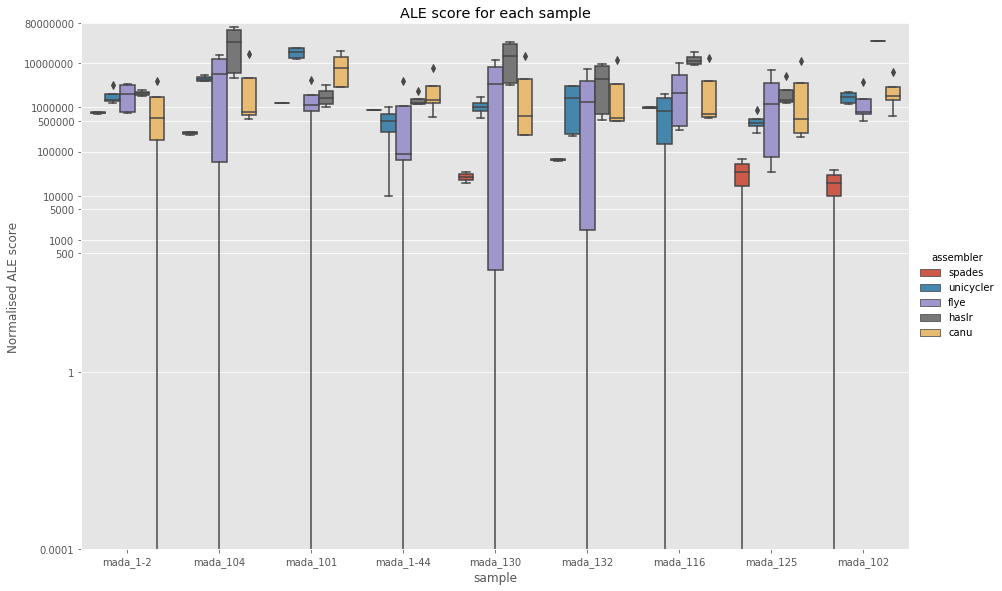
\includegraphics[width=1.0\textwidth]{Appendix1/Figs/ale_score.png}
\centering
\caption{The normalised assembly likelihood evaluation (ALE) score (Y-axis) for each sample (X-axis), coloured by assembly tools. ALE score is a metric describing the likelihood of an assembly. The normalisation is done by subtracting the assembly's score from the maximum (best) score for that sample, giving a relative probability of correctness. Each box represents different technologies and polishing status for each assembler.}
\label{fig:ale_score}
\end{figure}

\subsection{Disagreement rate}
\label{app:asm_disagree}

The disagreement rate is an approximation of the per-base accuracy of the assembly. We map Illumina reads to the assembly with \vrb{bwa mem} and calculate what proportion of positions do 90\% of the reads agree with the assembly nucleotide.  

In 7 of 9 samples, a \vrb{HASLR} assembly had the lowest disagreement rate, followed by \vrb{unicycler} having the minimum in 2. Polished genomes produced the lowest disagreement rate in 8/9 samples, and \ont{}-based assemblies had the best accuracy in 6/9 samples. While it is not so surprising that assemblies polished with Illumina reads have a lower disagreement rate, it is unexpected that \ont{} would produce more accurate assemblies (\autoref{fig:disagree_rate}). One caveat to keep in mind here is that there is an element of overfitting to this metric; we assess using Illumina, and so naturally, assemblies polished with Illumina produce better results. That is not to say this statistic is void, but that it should be used cautiously and not in isolation.

\begin{figure}
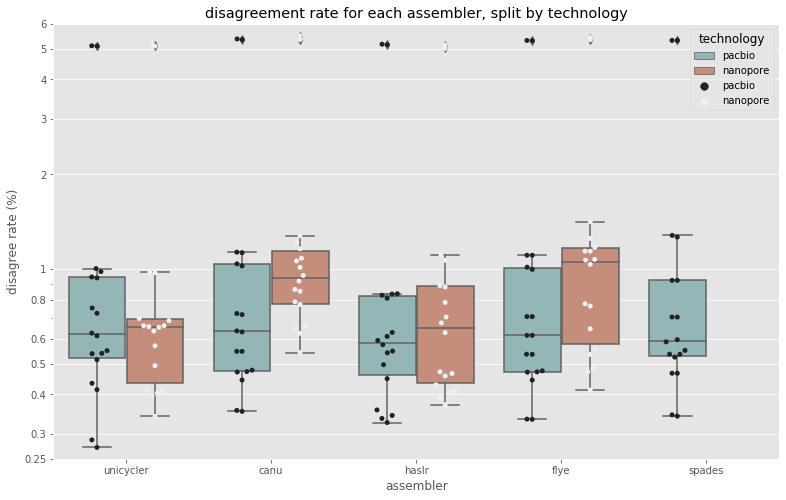
\includegraphics[width=1.0\textwidth]{Appendix1/Figs/disagree_rate.png}
\centering
\caption{The disagreement rate (y-axis) for each assembler (x-axis), coloured by the sequencing technology. Disagreement rate is the percentage of sites in the assembly where Illumina reads do not have at least 90\% quorum. Each box/point represents different samples and polished status for the relevant assembler/technology combination.}
\label{fig:disagree_rate}
\end{figure}

As part of calculating the disagreement rate, we also produce a BED file listing all positions with less than 90\% agreement. This BED file can be used as a genome mask when using the assembly for later analysis.

\subsection{Number of contigs}

As \mtb{} has only a single circular chromosome, for an assembly to be structurally complete, there should only be a single contig in the final assembly. However, it is not always appropriate for an assembly method to produce a single contig as data quality, depth of sequencing, read length, and repetitive content of the genome can hamper this goal. Conversely, receiving a single contig as output is no guarantee of its quality for similar reasons to the multi-contig scenario. For this benchmark, considered in conjunction with the other metrics, the number of contigs can be a helpful datum for selecting our favoured assembly. If an assembly has a single contig and scores well on other metrics, we would be more inclined to choose it over another assembly with similar metrics but many more contigs.

Across all combinations of assembly conditions, \vrb{spades} (8/18), \vrb{flye} (18/32) and \vrb{canu} (16/32) produced far more single-contig assemblies than the hybrid methods (\autoref{fig:num_contigs}). \vrb{unicycler} produced no single-contig genomes, whilst \vrb{HASLR} yielded only 2/32. When considering sequencing technology, PacBio (26/72) had many more single-contig assemblies than \ont{} (10/72). Note, \vrb{spades} assemblies use all three technologies and are not considered in the technology single-contig totals.

\begin{figure}
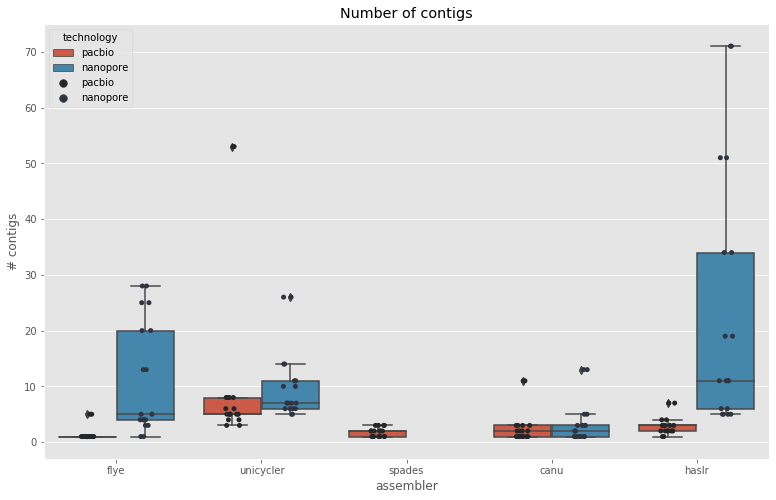
\includegraphics[width=1.0\textwidth]{Appendix1/Figs/num_contigs.png}
\centering
\caption{The number of contigs (Y-axis) produced from each assembly (X-axis), coloured by sequencing technology. Each box/point represents different samples and polished status for the relevant assembler-technology combination.}
\label{fig:num_contigs}
\end{figure}

\subsection{Length of assembly}

As mentioned earlier, comparing assemblies to the \mtb{} reference genome (H37Rv) is not appropriate due to lineage differences. However, assembly length/size can be used as an aid for selection. The size of any lineage's genome is not expected to differ from the reference by more than \texttildelow 30 kilobases \cite{kato2001}. Considering the genome size in addition to the disagreement rate is particularly informative. It would be easy for an assembly method to produce very accurate per-base contigs by refusing to produce sequences for "harder" parts of the genome. While such an assembly would score well on the disagreement rate, it would not do so well when considering how close it is to the expected genome size. The length of the assembly also clearly shows when a method is outputting \emph{too much} sequence.

When comparing each assembly to H37Rv, we found a fairly even spread across assemblers for the closest size to H37Rv. For 3/9 samples, \vrb{canu} has the smallest size difference, followed by \vrb{spades} (2/9), \vrb{unicycler} (2/9), \vrb{HASLR} (1/9) and \vrb{flye} (1/9). An honourable mention should be made of \vrb{flye} and \vrb{spades} as they had much lower variation in size compared to the other approaches. In terms of sequencing technology, in 6/9 samples, PacBio produced the genome size closest to H37Rv. Polished assemblies had the closer size in 5/9 samples.

\begin{figure}
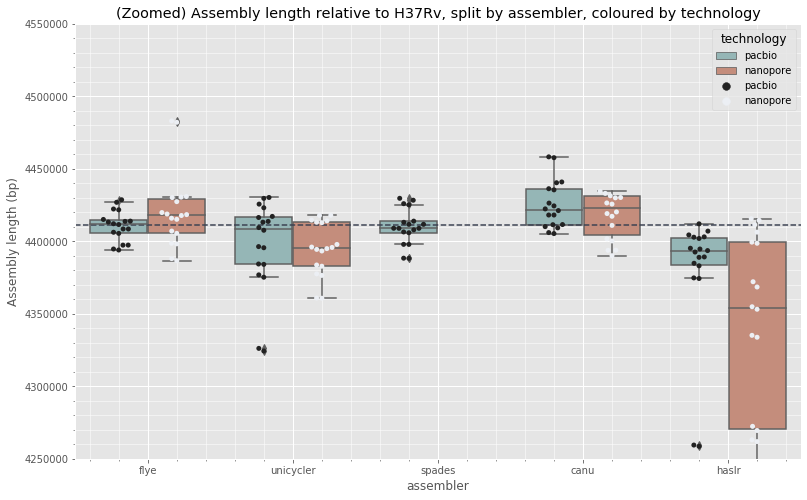
\includegraphics[width=1.0\textwidth]{Appendix1/Figs/asm_len.png}
\centering
\caption{Size/length (Y-axis; in base-pairs (bp)) of each assembly (X-axis), coloured by each sequencing technology. The horizontal dashed line represents the size of the \mtb{} reference genome (4,411,532bp). Each box/point represents different samples and polished status for the relevant assembler-technology combination. Note: the Y-axis has been limited to allow for greater resolution of similarity to the H37Rv size}
\label{fig:asm_len}
\end{figure}

\subsection{Contamination detection}

The decontamination step in the assembly pipeline revealed that one sample, \vrb{mada\_1-2}, contained contigs from three different species: \textit{Mycobacterium intracellulare}, \textit{Dermacoccus nishinomiyaensis}, and \mtb{}. These contigs were all at sufficient coverage to not be considered background noise. For the assembly assessment analysis, only the contigs from \mtb{} were used. However, this sample is an outlier in almost all the assessment metrics in the previous sections. Given this profuse contamination, \vrb{mada\_1-2} will not be used in any analysis where these assemblies are used for truth validation purposes.

\subsection{Summary}

In conclusion, considering all assessment metrics, \vrb{flye} and \vrb{spades} assemblies were consistently the better performing methods across all of the criteria outlined in this section. As most of the validation analyses that these assemblies will be used for involve comparing Illumina and \ont{} data to a "neutral truth", the unpolished PacBio CCS assemblies from \vrb{flye} were selected for use. The differences between the polished and unpolished CCS assemblies were negligible. Therefore, they did not outweigh the benefit of having a single-technology PacBio assembly that can be used as an unbiased reference point for comparing the other two technologies.

% ===========================================================

\section{Masking of the \mtb{} reference graph}
\label{app:mask}

We investigated three different strategies for masking the positions that go into the \mtb{} reference graph in \autoref{sec:tbprg}. The first was not to use a mask and apply all variants that passed all other filters in the \cryptic{} VCF. Compared to the final method we chose, this lead to the sparse \prg{} MSA step having a peak memory usage of 357GB (1.7 times more than \autoref{tab:build-prg}) and a wall clock time of 13.5 hours (compared to 1.25). The dense \prg{} MSA likewise saw higher memory usage (370GB) and wall clock time (44.6 hours). In addition, when updating these \prg{}s to include novel variants (\autoref{sec:pandora-filters}), the MSA stage took on the order of days to complete.

The second masking strategy was to remove the VCF positions that occur within the H37Rv genome mask mentioned in \autoref{sec:tbprg}. This approach would ensure there would be sequence covering the whole H37Rv genome within the reference graph. This approach yields construction times similar to those in \autoref{tab:build-prg}. However, this caused the novel variant discovery stage of \pandora{} to hit the seven-day compute node run limit for some samples. The cause of this huge increase can be explained by the fact that the positions within the mask are, by definition, repetitive (low complexity). As such, when \pandora{} initiates \denovo{} variant discovery in these sections of the genome, the path enumeration step outlined in \autoref{sec:path-enum} gets caught in cycles within the de Bruijn graph - a limitation outlined in \autoref{sec:denovo-limits}.

The third strategy is the one we ended up using - removing loci with $\ge 30\%$ of their positions in the mask. The 30\% figure was settled on as it provided a good balance between losing sections of the H37Rv genome (see \autoref{fig:loci-mask}) and providing acceptable computational performance for all steps in the reference graph construction and \pandora{} variant-calling pipeline.

\begin{figure}
     \centering
     \begin{subfigure}[b]{0.475\textwidth}
         \centering
         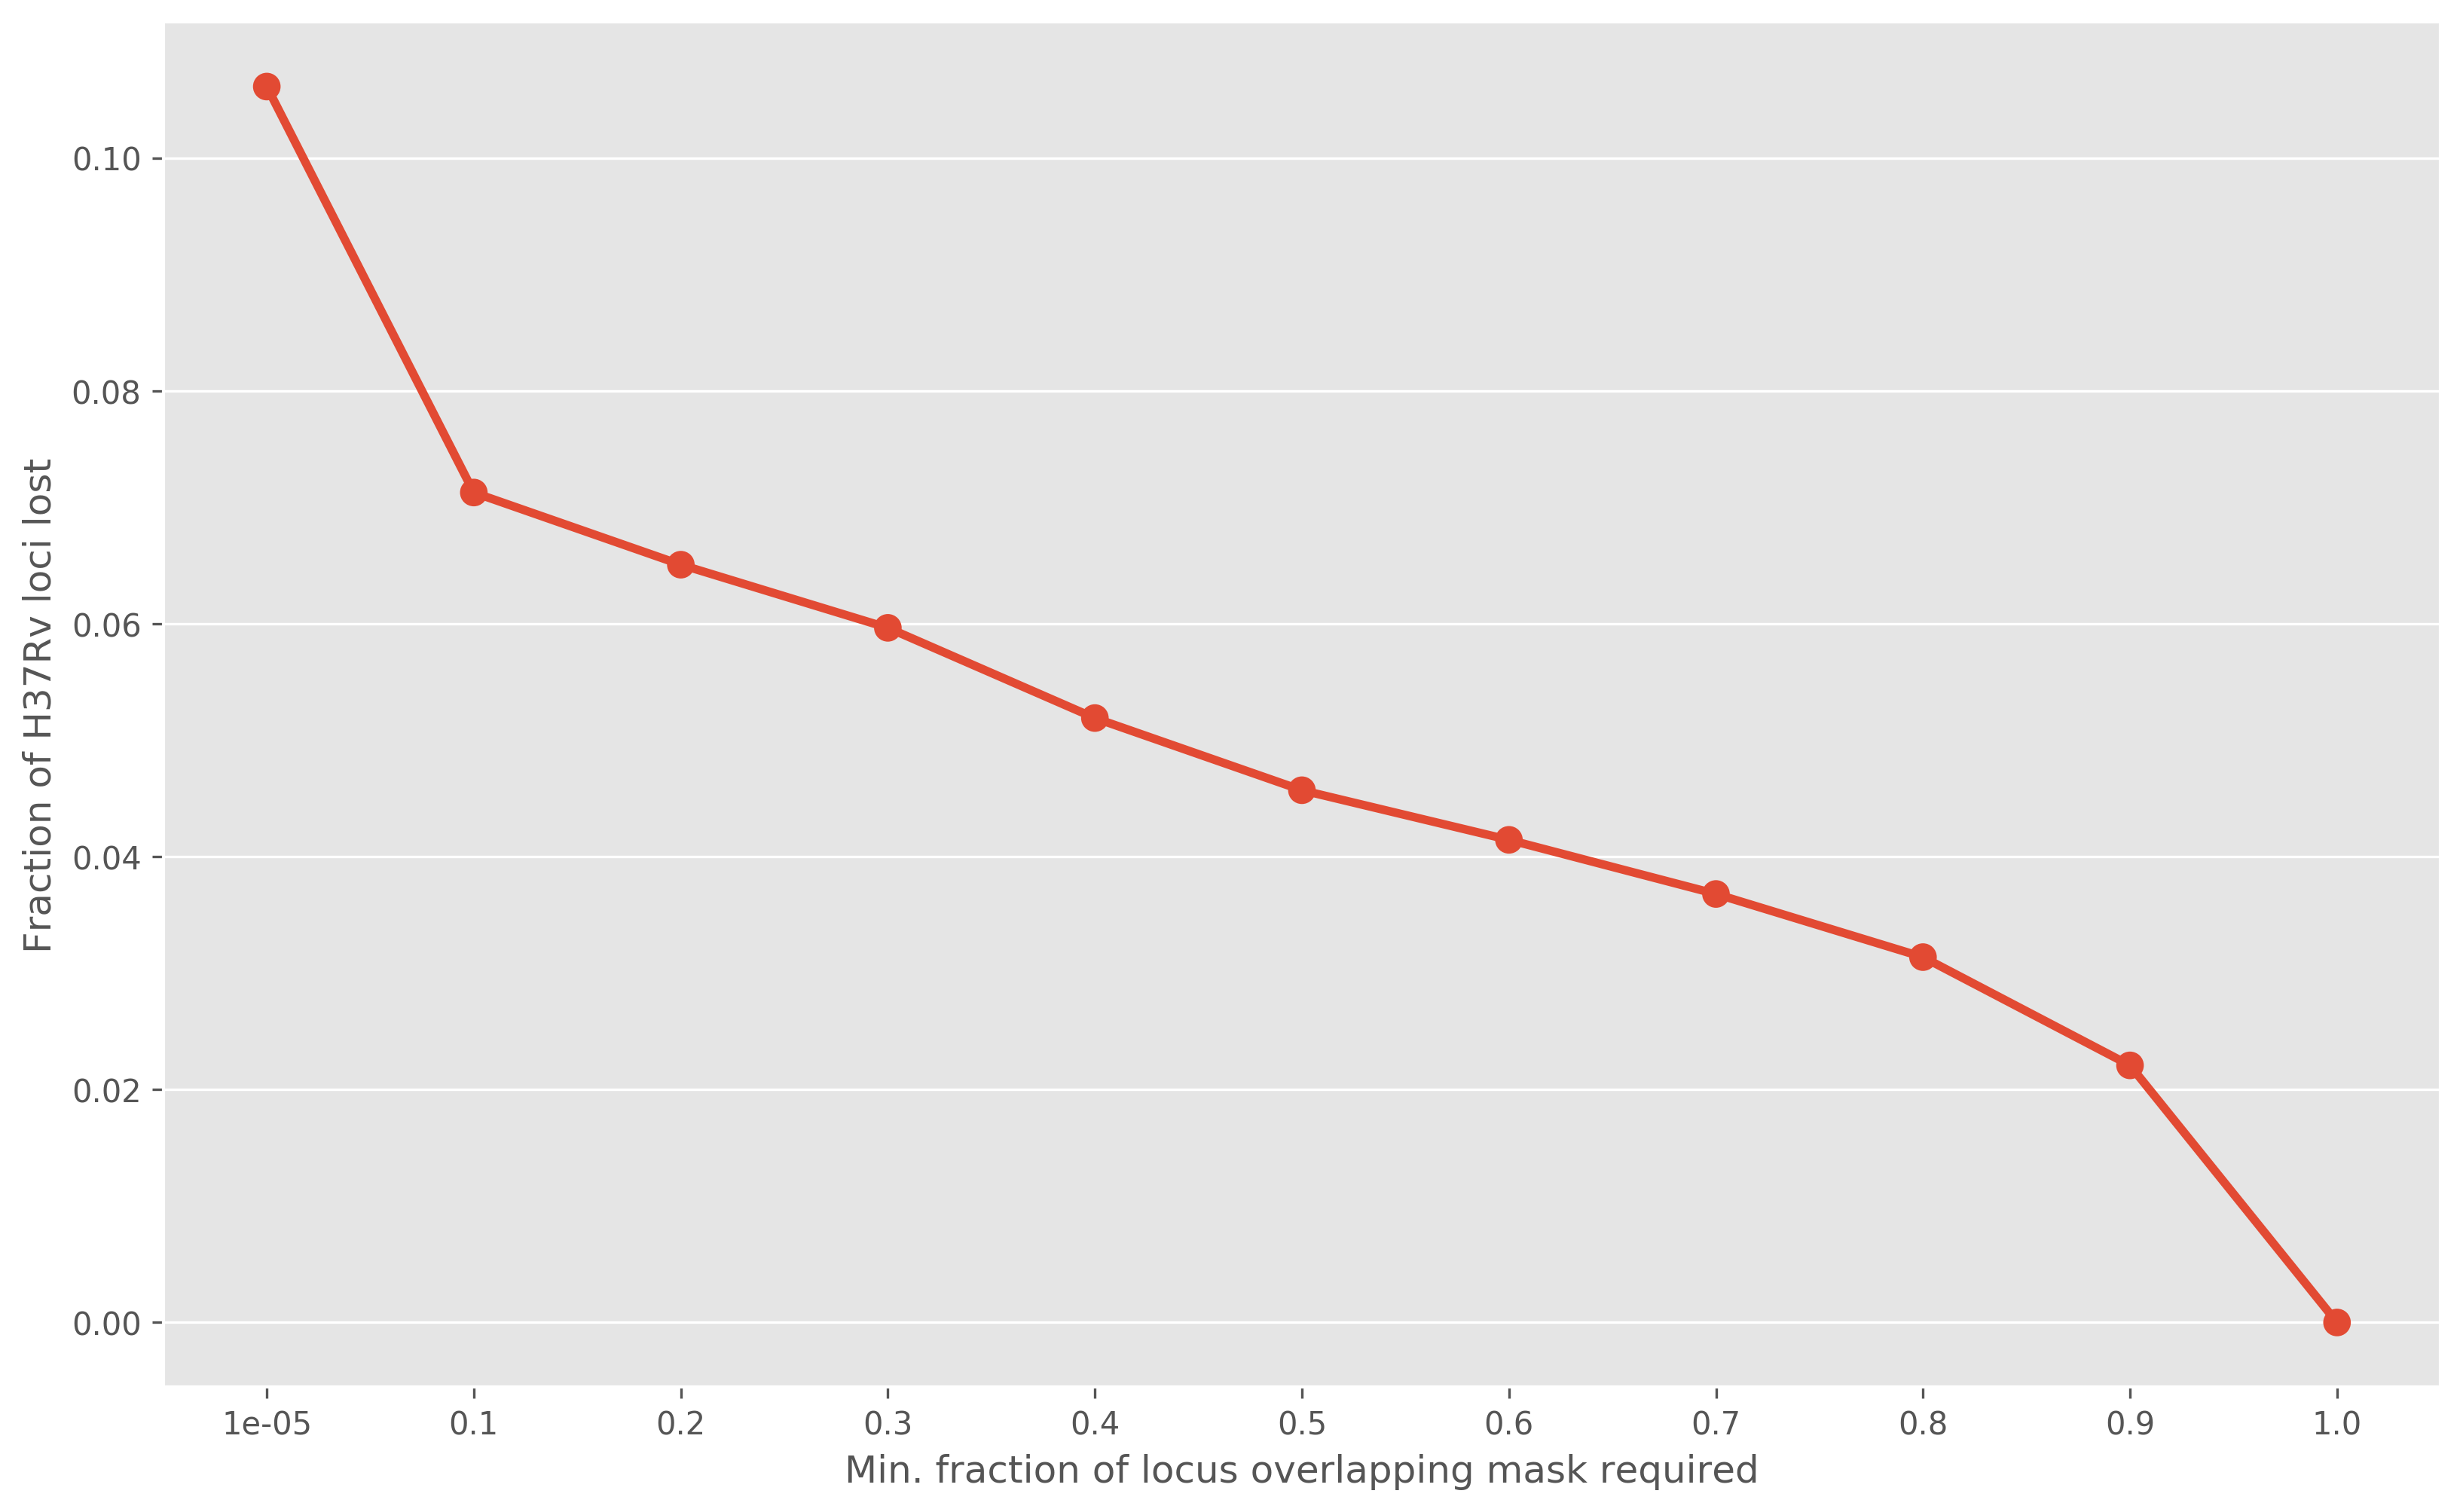
\includegraphics[width=\textwidth]{Appendix1/Figs/loci-lost.png}
         \caption{}
         \label{fig:loci-lost}
     \end{subfigure}
     \hfill
     \begin{subfigure}[b]{0.475\textwidth}
         \centering
         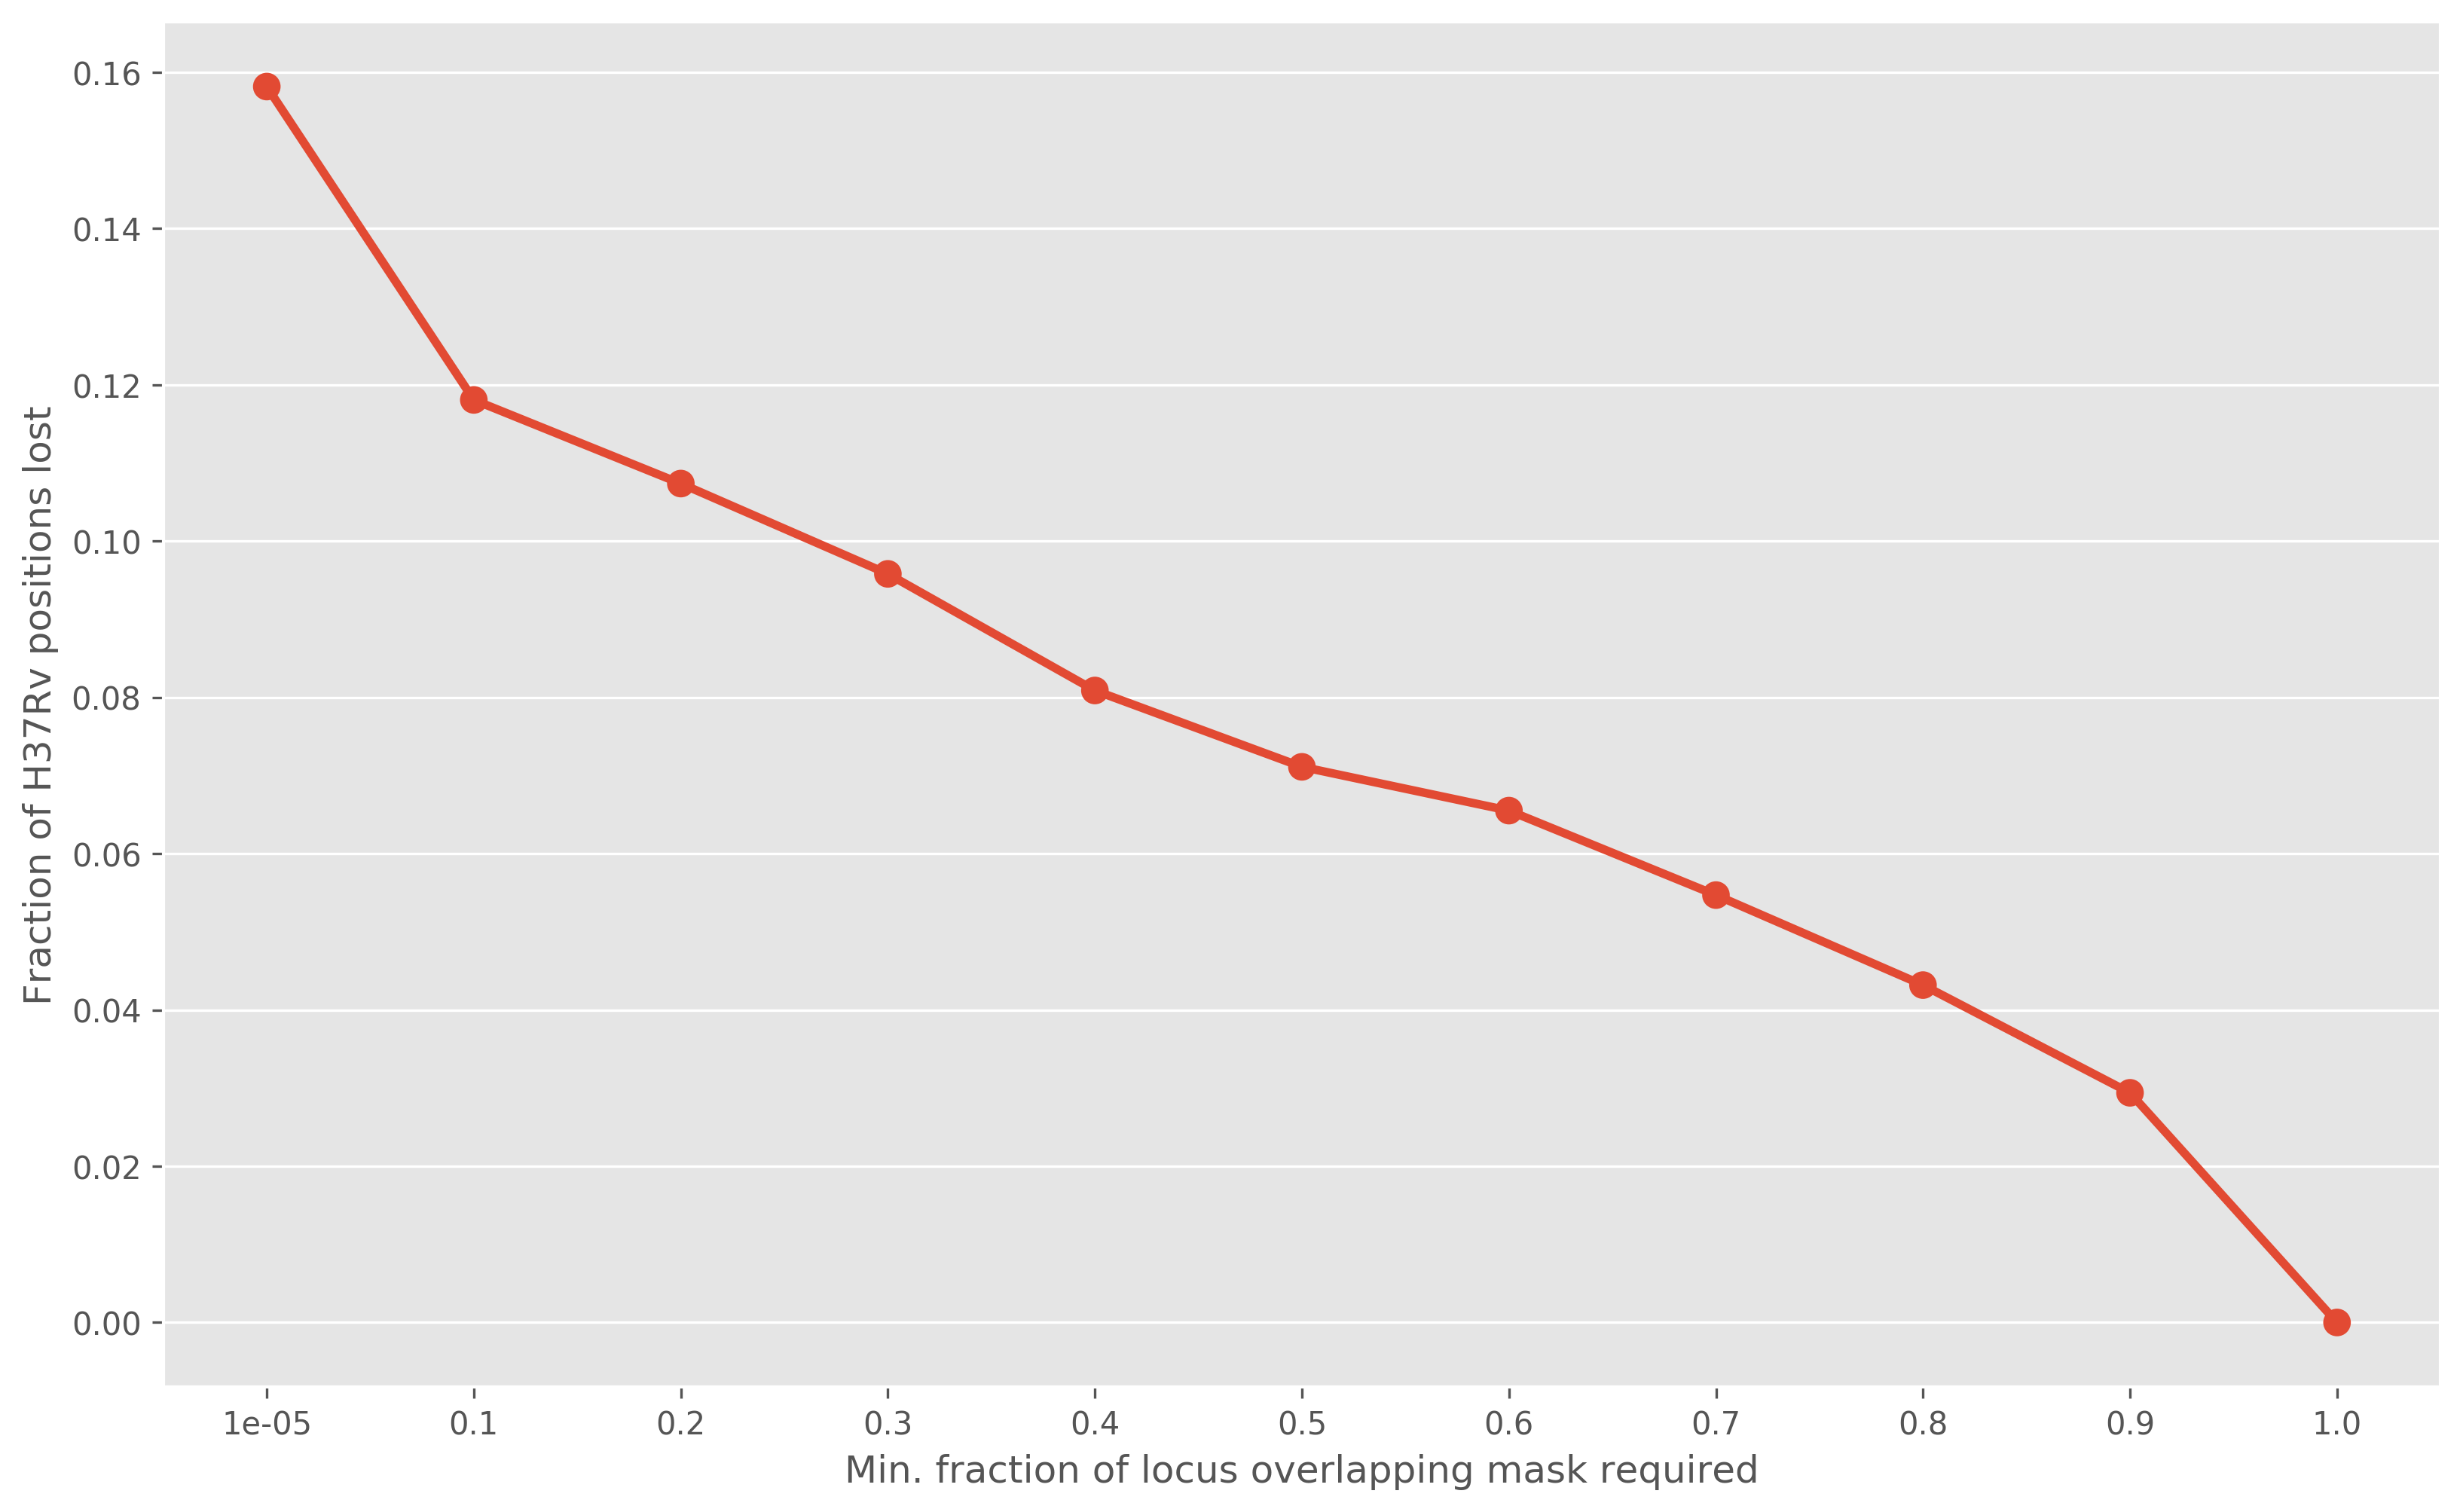
\includegraphics[width=\textwidth]{Appendix1/Figs/pos-lost.png}
         \caption{}
         \label{fig:pos-lost}
     \end{subfigure}
        \caption{\textbf{a)} Proportion of loci lost (y-axis) when removing those with a certain fraction (x-axis) of their positions within the genome mask. \textbf{b)} Proportion of total genome positions lost (y-axis) when removing loci with a certain fraction (x-axis) of their positions within the genome mask.}
        \label{fig:loci-mask}
\end{figure}

% ===========================================================

\section{Precision and recall of all variant calls from \pandora{}}
\label{app:pandora-all-vars}

Although we only use SNPs for identifying transmission clusters (\autoref{sec:map-var-calls}), we also assessed \pandora{} variant calls for all variants - SNPs and indels up to a length of 20bp. The precision and recall using the same filters as in \autoref{sec:map-var-calls} are shown in \autoref{fig:pandora-filters-all}. We did this for the sake of future work that might be interested in using \pandora{} indel calls, such as predicting drug resistance. Again, the sparse \prg{} gave better precision and recall than the dense one. The use of all variants leads to a median recall improvement to 75.48\% (all filters) - up 3.49\% from SNPs only. On the other hand, precision sees a drop to 95.90\% (median) when assessing all variants - compared to 100\% for SNPs only. Given the large drop in precision, it is clear that \pandora{} indel-calling needs further improvement. However, indel-calling (deletions especially) is a known limitation of \ont{} \cite{jain2018,wick2019} and others have seen precision drops when adding indels to the evaluation \cite{clair2020}.

\begin{figure}
\begin{center}
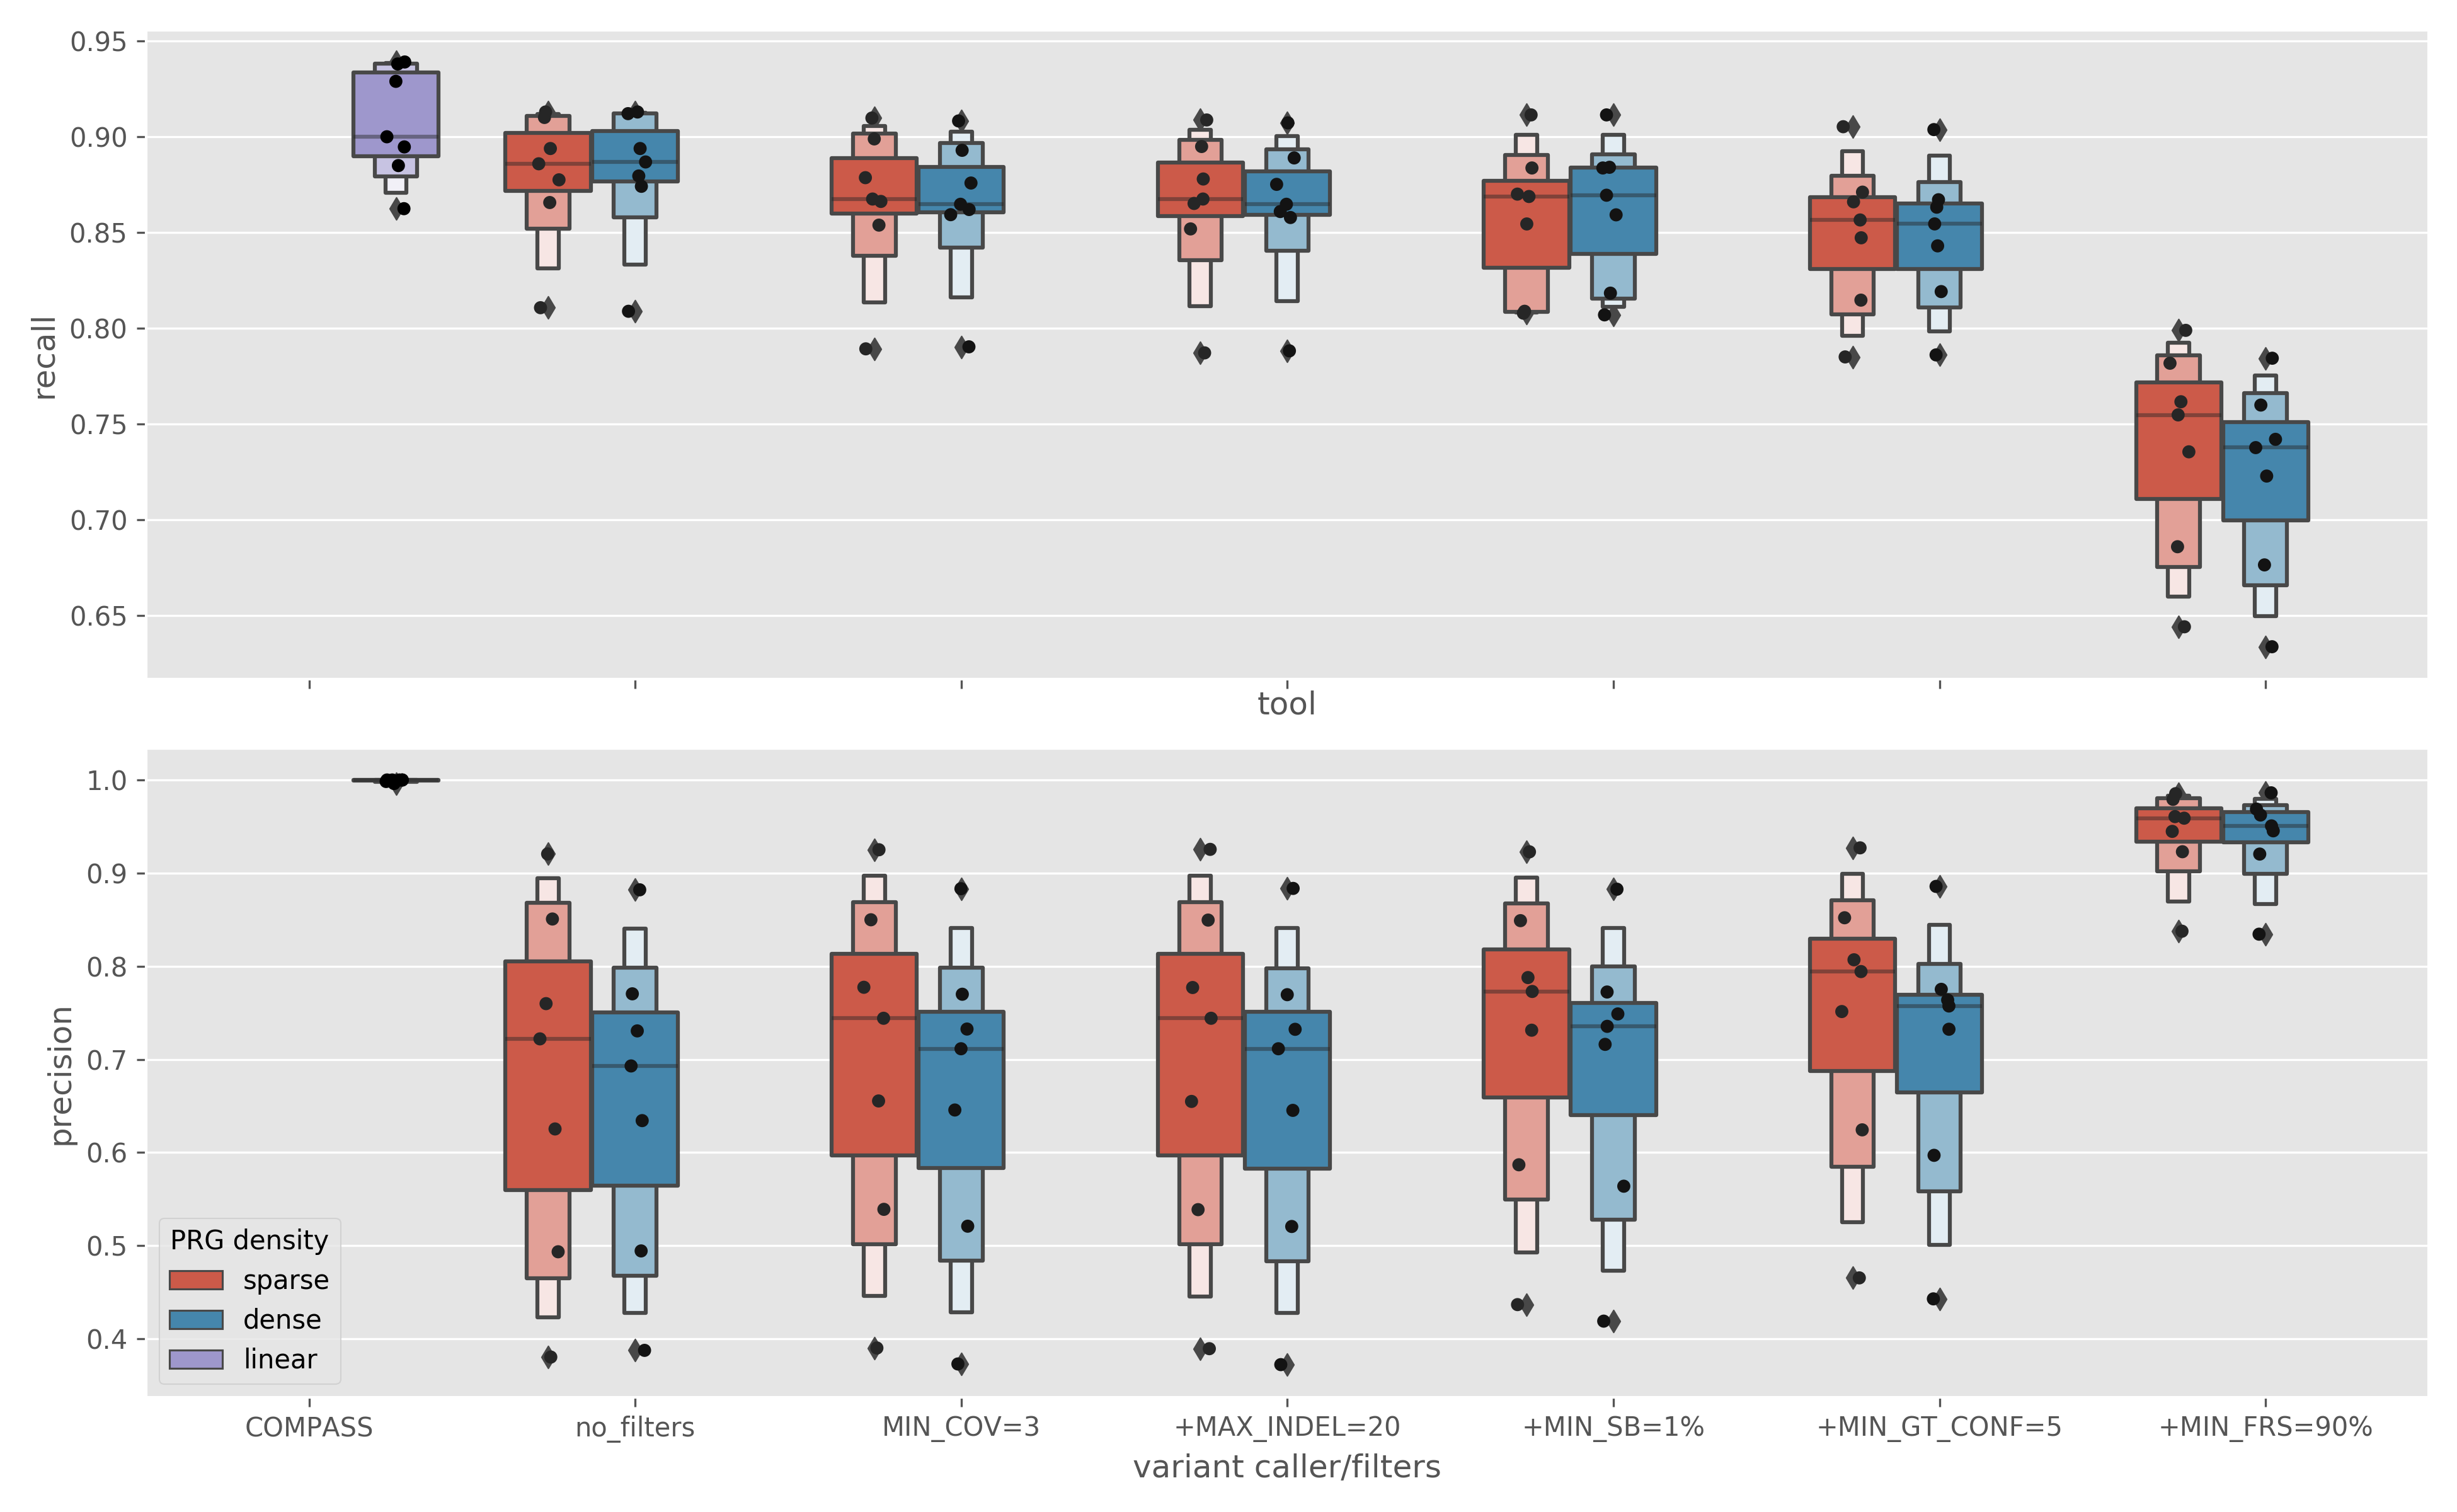
\includegraphics[width=0.90\columnwidth]{Appendix1/Figs/pandora-precision-recall-filters-all-variants.png}
\caption{{Precision (bottom) and recall (top) of SNPs for COMPASS (purple) and all variants (maximum indel length of 20bp) for \pandora{} with sparse (red) and dense (blue) \prg{}s. The \pandora{} boxes start with no filters on the left, with each box moving to the right adding a filter to the previous box. The COMPASS box is a reference to the precision and recall of Illumina variant calls. Linear PRG density refers to the fact that COMPASS uses a single, linear reference genome as opposed to \pandora{}, which uses a genome graph. The black points refer to single data points for the seven samples used. MIN\_COV=minimum depth of coverage; MIN\_SB=minimum strand bias; MIN\_GT\_CONF=minimum genotype confidence score; MIN\_FRS=minimum fraction of read support.
{\label{fig:pandora-filters-all}}%
}}
\end{center}
\end{figure}

% ===========================================================

\section{An illustrated example of cluster similarity metrics}
\label{app:cluster-example}

\autoref{sec:cluster-similarity} outlines three metrics - SACR, SACP and XCR - for evaluating the similarity between two different strategies for transmission clustering. In order to provide the reader with greater intuition for the purpose of each metric, we present an illustrated example in \autoref{fig:cluster-example}. 

We take \autoref{fig:example-truth} to be the truth clusters and \autoref{fig:example-test} to be test clusters. These are akin to Illumina and \ont{} clusters, respectively, in \autoref{sec:cluster-similarity}). The individual recall and precision values (defined in \autoref{eq:recall} and \autoref{eq:precision}) for each sample in \autoref{fig:example-truth} are shown in \autoref{tab:cluster-example}. SACR and SACP (defined in \autoref{eq:sacr} and \autoref{eq:sacp}) are \emph{sample-averaged}, so their values for this example are 0.82 and 0.83 respectively. 

To highlight the objective of SACR, we use the truth and test clusters containing the sample $F$. Samples $F$, $G$, $H$ and $I$ are shared between both, but $J$ is missing from the test cluster. To calculate the individual recall for $F$, we take the intersection size of the truth and test clusters it exists in and divide it by the size of the truth cluster - $\frac{4}{5}=0.8$. We do the same for the precision of sample $D$, expect we divide by the size of the test cluster - giving $\frac{2}{3}=0.66$. 

The relevance of the XCR metric is best exemplified by the test cluster containing samples $L$ and $M$. As we calculate SACR and SACP for all samples in the \emph{truth} clusters, these two samples would be ignored. However, they are samples that - according to the truth - should not be part of any cluster (singletons). Therefore, SACR and SACP cannot capture these extra clusterings if they do not contain clustered truth samples. XCR covers this limitation and is the proportion of singletons in the truth that are clustered in the test (see \autoref{eq:xcr}). As \autoref{fig:cluster-example} does not show singletons, let us pretend there are 20 singletons in the truth (including samples $L$ and $M$). This would give an XCR of $2/20=0.1$.

\begin{figure}
     \centering
     \begin{subfigure}[b]{0.4\textwidth}
         \centering
         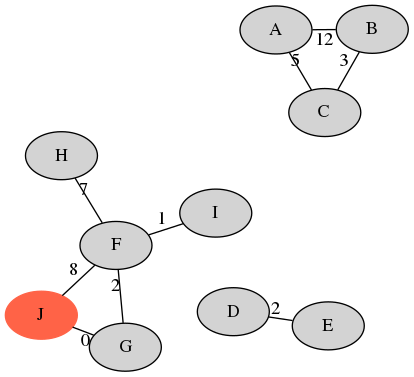
\includegraphics[width=\textwidth]{Appendix1/Figs/illumina-cluster-example.png}
         \caption{}
         \label{fig:example-truth}
     \end{subfigure}
     \hfill
     \begin{subfigure}[b]{0.4\textwidth}
         \centering
         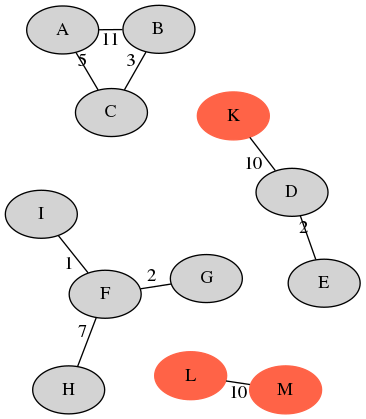
\includegraphics[width=\textwidth]{Appendix1/Figs/ont-cluster-example.png}
         \caption{}
         \label{fig:example-test}
     \end{subfigure}
        \caption{Illustrative examples of transmission clustering. \textbf{a)} represents truth clusters, while \textbf{b)} is clustering from some "test" method we would like to compare to \textbf{a}. The nodes represent samples with the numbers on the edges connecting them indicating the distance between those two samples. The red nodes indicate samples with a clustering disparity between the two clusterings.}
        \label{fig:cluster-example}
\end{figure}

\begin{table}
\centering
\begin{tabular}{|c|c|c|}
sample & recall & precision \\
\hline
A      & 1.0    & 1.0       \\
B      & 1.0    & 1.0       \\
C      & 1.0    & 1.0       \\
D      & 1.0    & 0.66      \\
E      & 1.0    & 0.66      \\
F      & 0.8    & 1.0       \\
G      & 0.8    & 1.0       \\
H      & 0.8    & 1.0       \\
I      & 0.8    & 1.0       \\
J      & 0.0      & 0.0        
\end{tabular}
\caption{Cluster recall and precision results for each sample in \autoref{fig:cluster-example}.}
\label{tab:cluster-example}
\end{table}

% ===========================================================

\section{Selecting \ont{} SNP thresholds to define transmission clusters}
\label{app:dist-sweep}

In \autoref{sec:snp-dist}, we fit linear models that describe the relationship between the Illumina and \ont{} SNP distance between pairs of samples. Using the equations for each model, we can infer a \ont{} threshold ($y$) corresponding to a given Illumina threshold ($x$). Next, we investigate how well these model-based thresholds perform by using the cluster similarity metrics defined in \autoref{sec:cluster-similarity}. To assess the performance, we look at the SACR, SACP, and XCR for all threshold values surrounding the model-based threshold and see whether the model-based threshold performs best.

\subsection{BCFtools}

For the Illumina SNP thresholds 0, 2, 5, and 12, the corresponding \bcftools{} model-inferred thresholds are 1, 3, 5, and 10 (red vertical dashed lines in \autoref{fig:bcftools-dist-sweep}). Based on the threshold sweep in \autoref{fig:bcftools-dist-sweep}, the best SNP distance thresholds to use for \bcftools{} are deemed 0, 2, 5, and 11 as these provide the best balance between the three similarity metrics.

\begin{figure}
\begin{center}
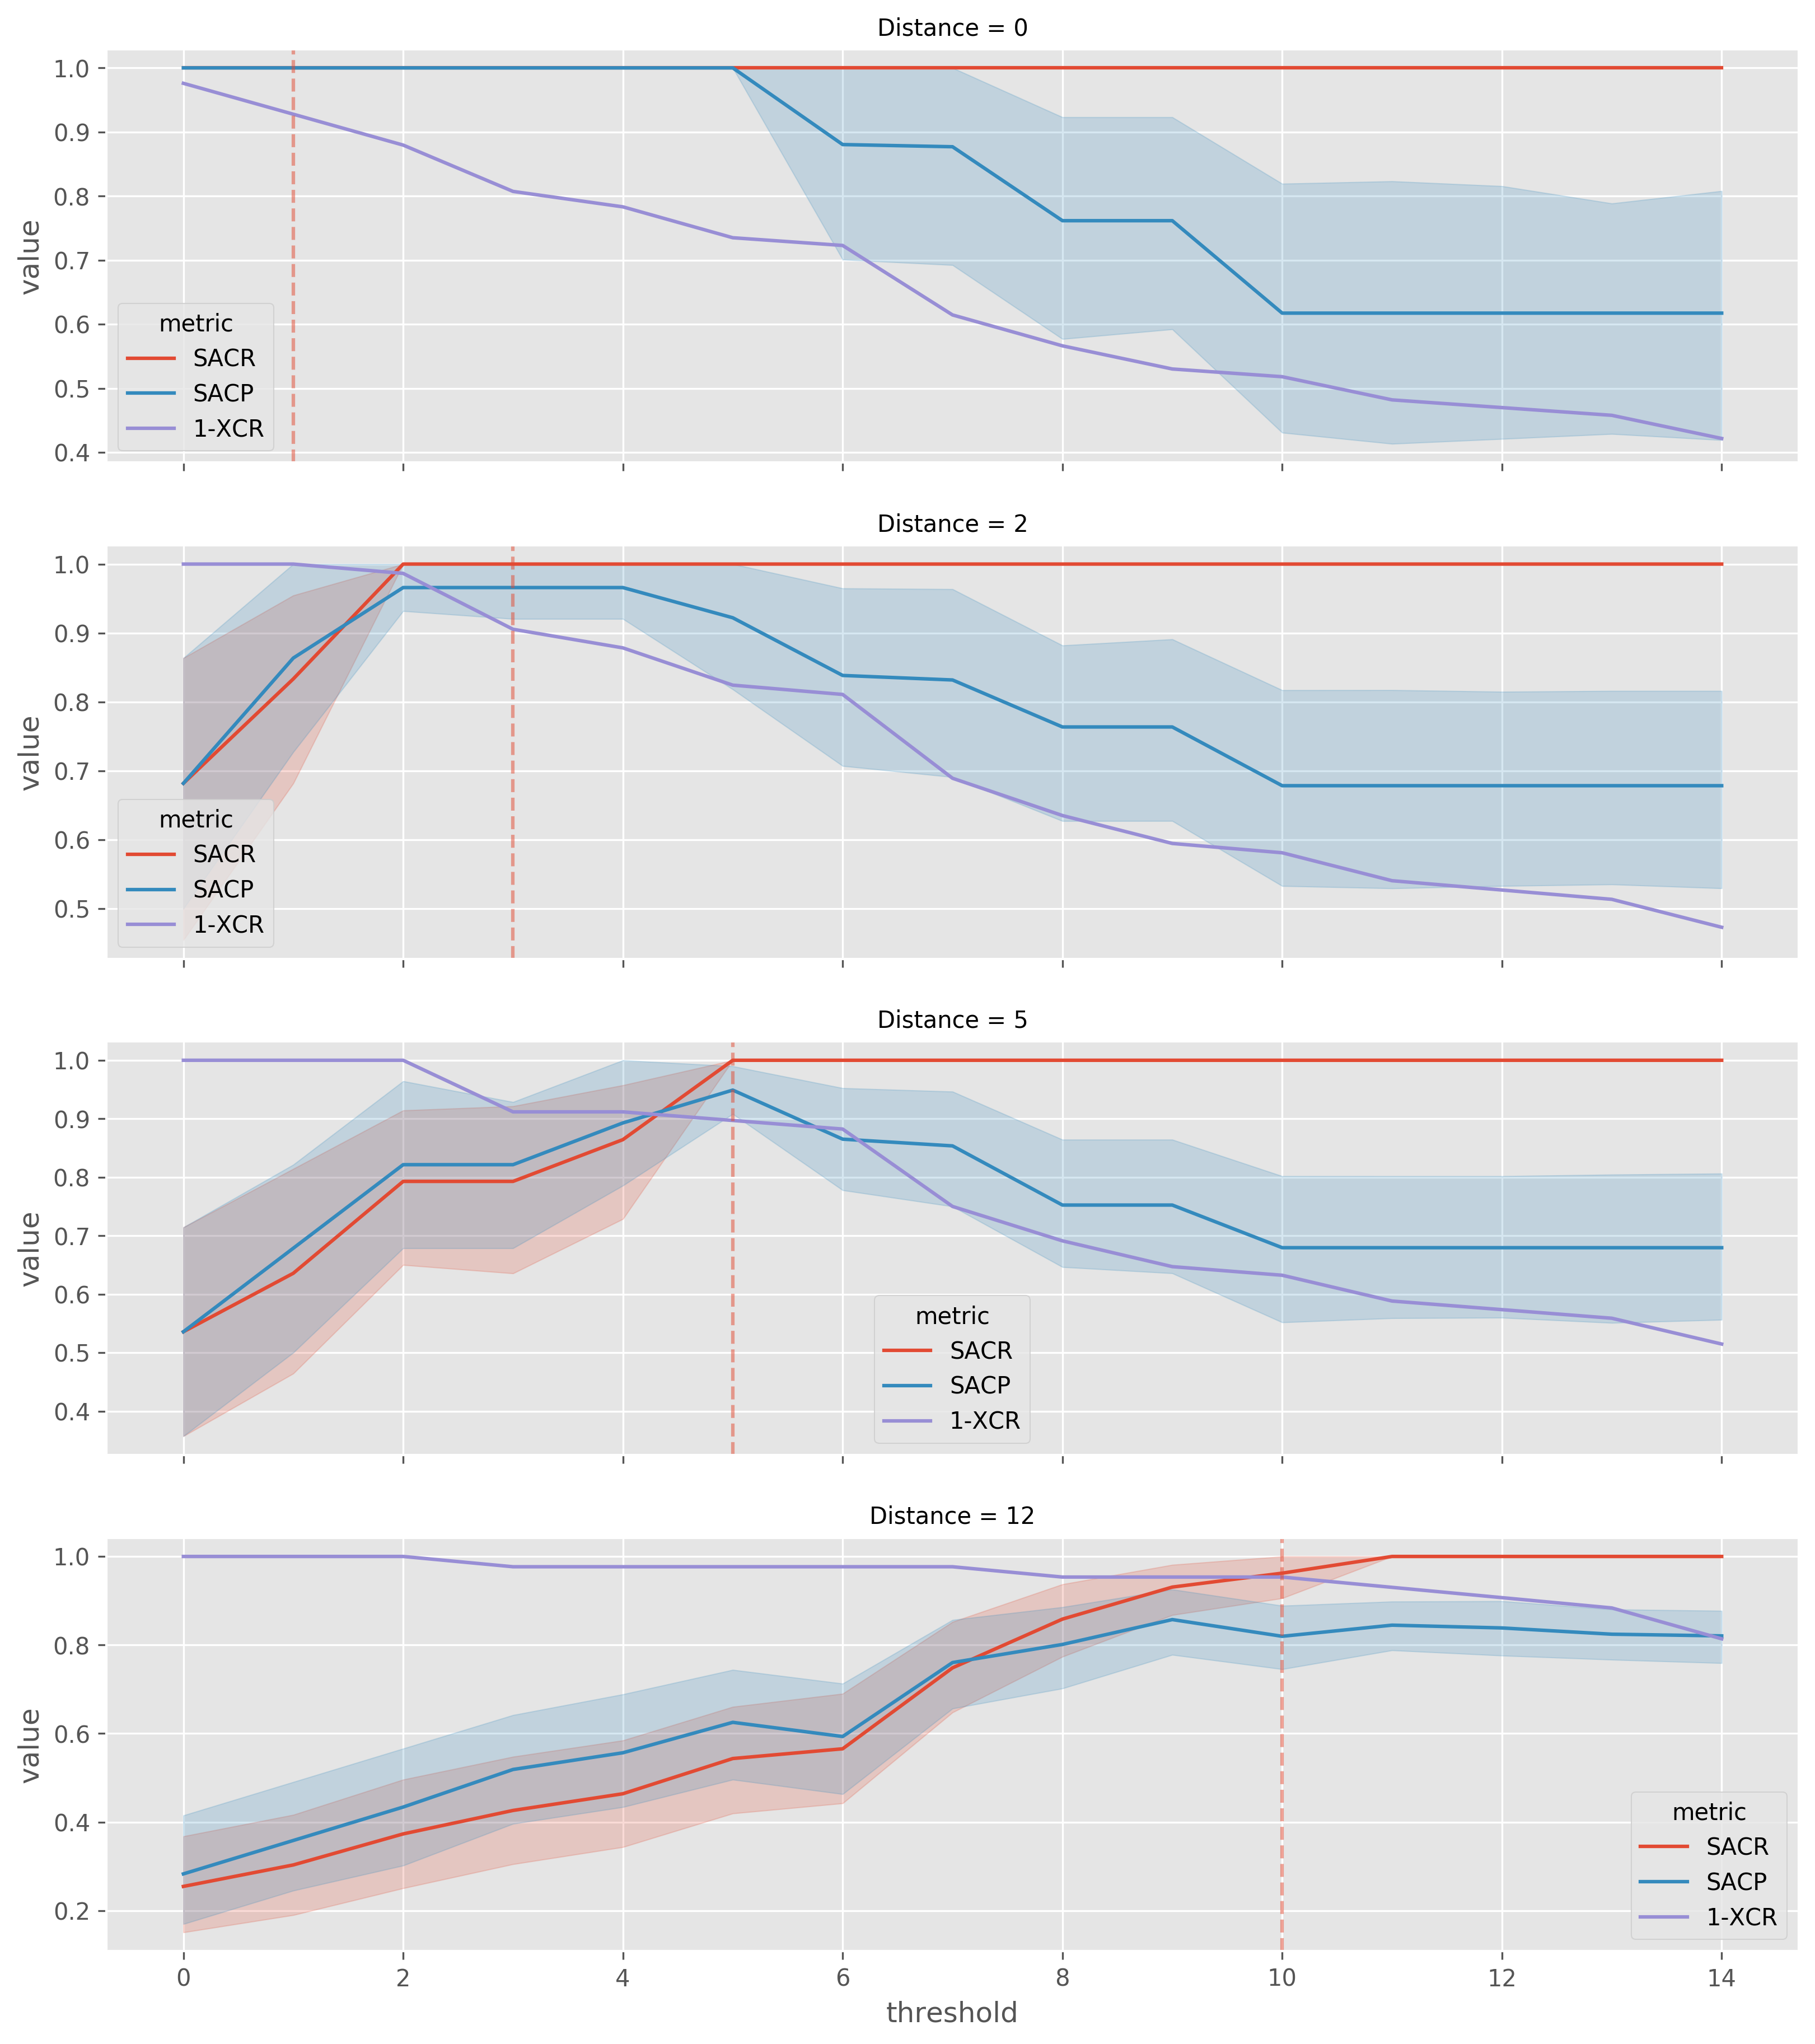
\includegraphics[width=0.90\columnwidth]{Appendix1/Figs/bcftools-threshold-sweep.png}
\caption{{Illumina and \ont{} (\bcftools{}) transmission cluster similarity for various SNP distance threshold. Each subplot compares the \ont{} clustering for the threshold on the x-axis to the Illumina clustering based on the distance (threshold) in the subplot title. SACR (red), SACP (blue), and $1-$XCR are represented by the lines with the band around the line indicating the 95\% confidence interval. The red, vertical, dashed lines indicate the model-based prediction of what the \ont{} SNP distance threshold should be based on the Illumina distance for that subplot.
{\label{fig:bcftools-dist-sweep}}%
}}
\end{center}
\end{figure}

\subsection{\pandora{} single-sample}

For the Illumina SNP thresholds 0, 2, 5, and 12, the corresponding \pandora{} single-sample model-inferred thresholds are 15, 17, 19, and 24 (red vertical dashed lines in \autoref{fig:map-dist-sweep}). Based on the threshold sweep in \autoref{fig:map-dist-sweep}, the best SNP distance thresholds to use for \pandora{} single-sample are deemed 16, 18, 18, and 27 as these provide the best balance between the three similarity metrics.

\begin{figure}
\begin{center}
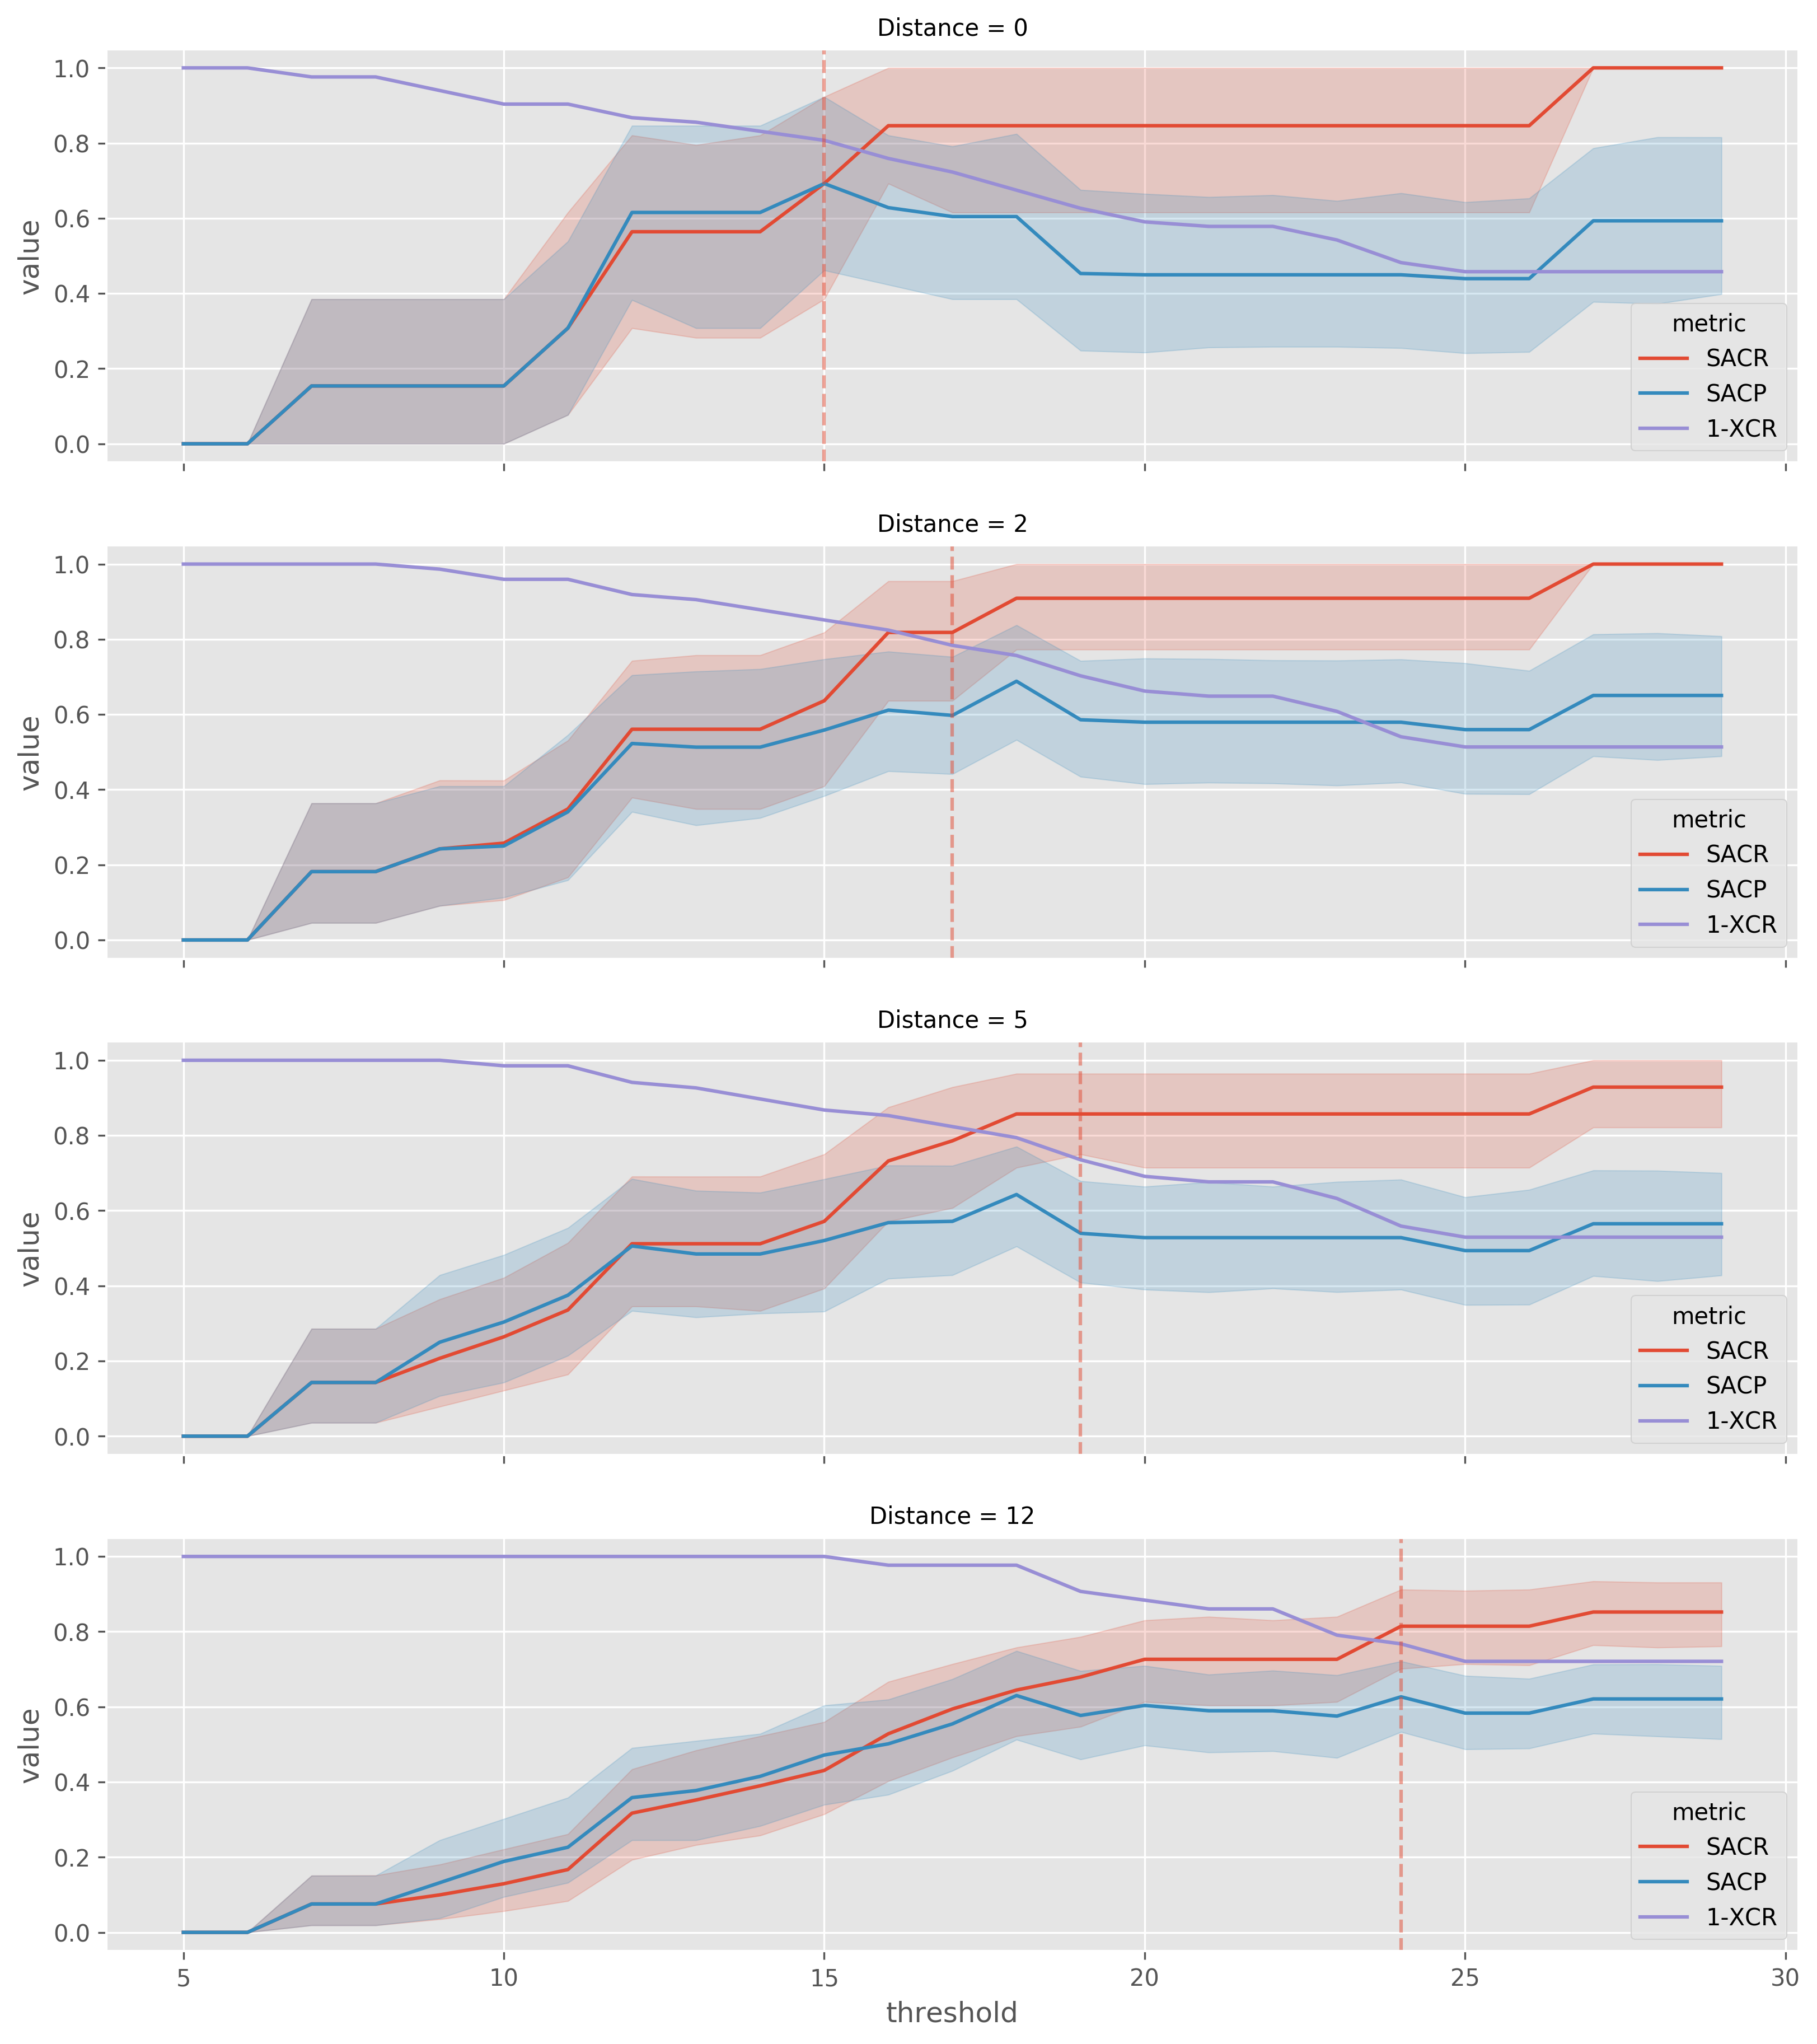
\includegraphics[width=0.90\columnwidth]{Appendix1/Figs/map-threshold-sweep.png}
\caption{{Illumina and \ont{} (\pandora{} single-sample) transmission cluster similarity for various SNP distance threshold. Each subplot compares the \ont{} clustering for the threshold on the x-axis to the Illumina clustering based on the distance (threshold) in the subplot title. SACR (red), SACP (blue), and $1-$XCR are represented by the lines with the band around the line indicating the 95\% confidence interval. The red, vertical, dashed lines indicate the model-based prediction of what the \ont{} SNP distance threshold should be based on the Illumina distance for that subplot.
{\label{fig:map-dist-sweep}}%
}}
\end{center}
\end{figure}

\subsection{\pandora{} multi-sample}

For the Illumina SNP thresholds 0, 2, 5, and 12, the corresponding \pandora{} multi-sample model-inferred thresholds are 0, 0, 1, and 4 (red vertical dashed lines in \autoref{fig:compare-dist-sweep}). Based on the threshold sweep in \autoref{fig:compare-dist-sweep}, the best SNP distance thresholds to use for \pandora{} multi-sample are deemed 0, 1, 3, and 7 as these provide the best balance between the three similarity metrics.

\begin{figure}
\begin{center}
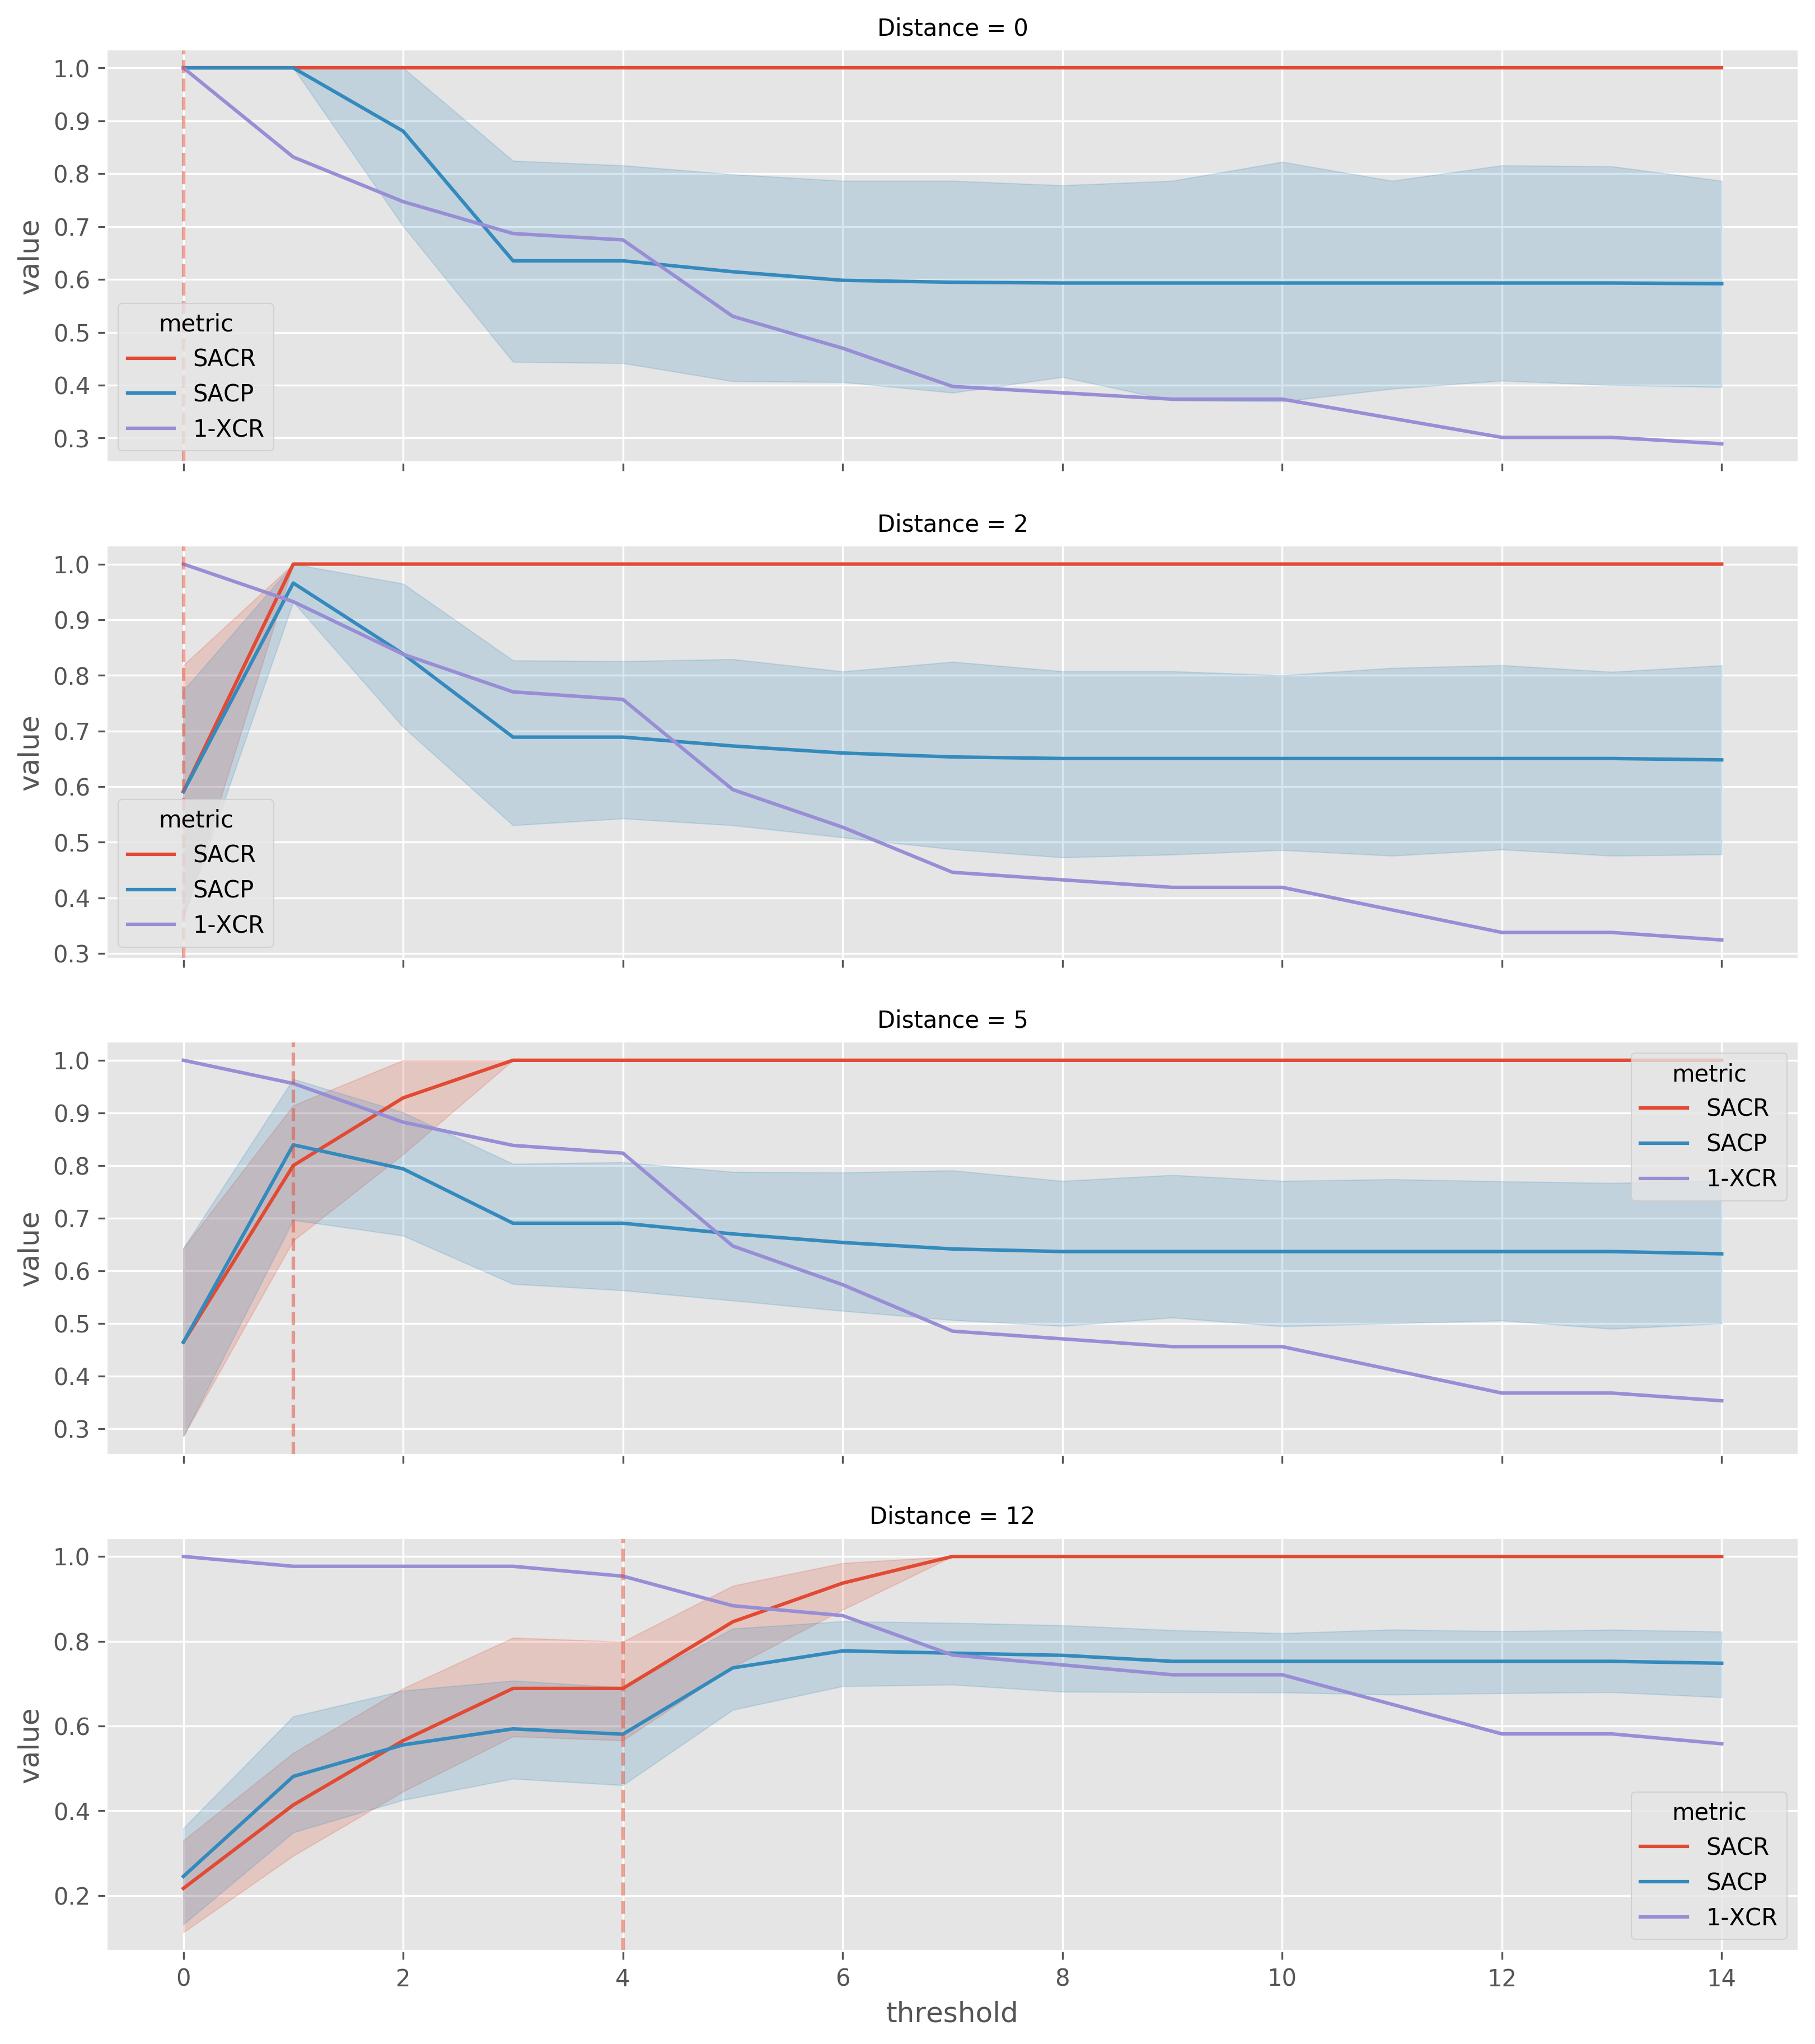
\includegraphics[width=0.90\columnwidth]{Appendix1/Figs/compare-threshold-sweep.png}
\caption{{Illumina and \ont{} (\pandora{} multi-sample) transmission cluster similarity for various SNP distance threshold. Each subplot compares the \ont{} clustering for the threshold on the x-axis to the Illumina clustering based on the distance (threshold) in the subplot title. SACR (red), SACP (blue), and $1-$XCR are represented by the lines with the band around the line indicating the 95\% confidence interval. The red, vertical, dashed lines indicate the model-based prediction of what the \ont{} SNP distance threshold should be based on the Illumina distance for that subplot.
{\label{fig:compare-dist-sweep}}%
}}
\end{center}
\end{figure}

\vspace{\baselineskip}
\noindent
In summary, the model-based thresholds chosen for the \ont{} variant callers are not the best-performing. Therefore, for all further transmission cluster work, the hand-picked thresholds are used instead.

% ===========================================================

\section{Transmission clusters}

These are the transmission clusters produced by each variant caller in \autoref{sec:eval-clusters}.

\begin{figure}
     \centering
     \begin{subfigure}[b]{0.45\textwidth}
         \centering
         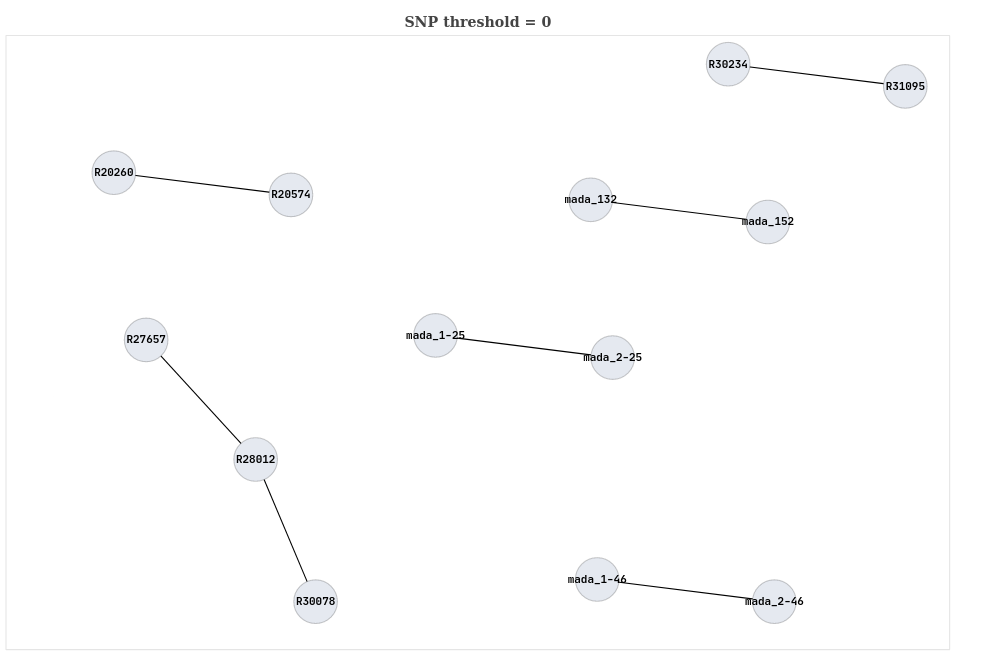
\includegraphics[width=\textwidth]{Appendix1/Figs/compass_clusters_t0.png}
         \caption{}
     \end{subfigure}
     \hfill
     \begin{subfigure}[b]{0.45\textwidth}
         \centering
         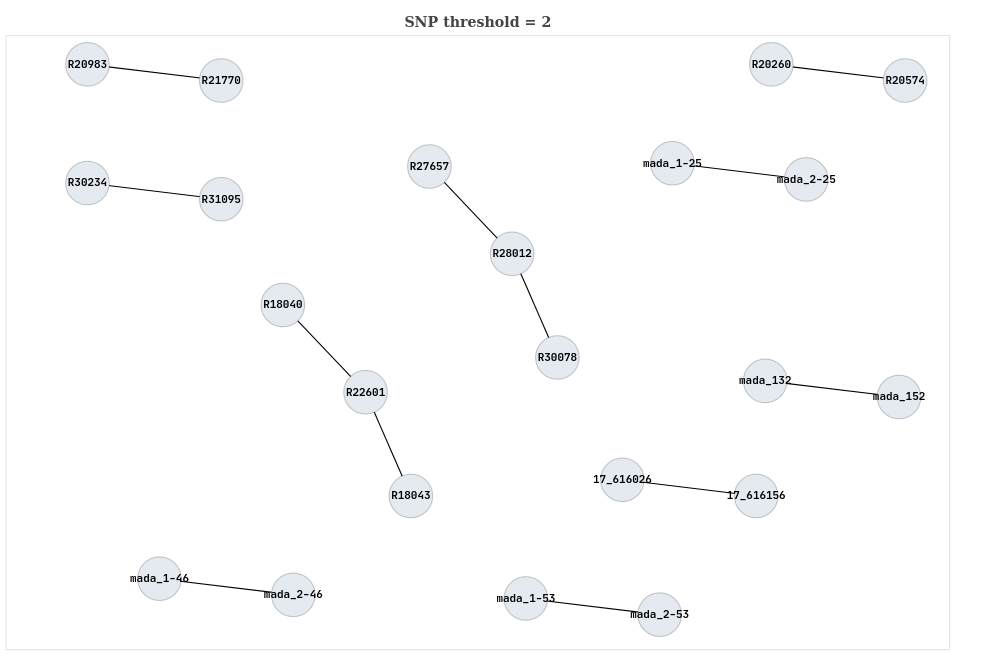
\includegraphics[width=\textwidth]{Appendix1/Figs/compass_clusters_t2.png}
         \caption{}
     \end{subfigure}
     \begin{subfigure}[b]{0.45\textwidth}
         \centering
         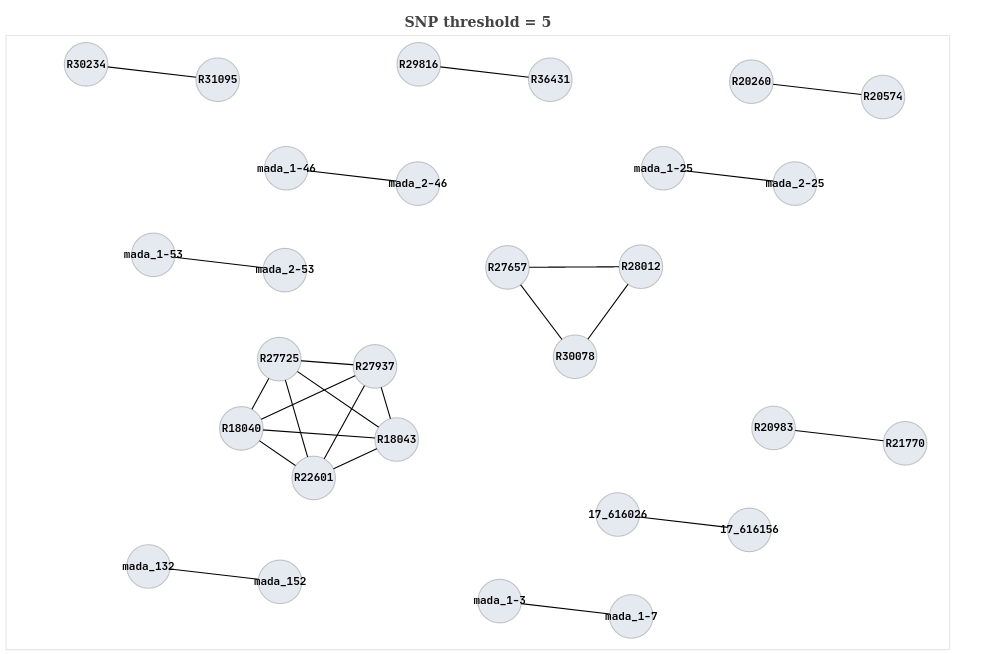
\includegraphics[width=\textwidth]{Appendix1/Figs/compass_clusters_t5.png}
         \caption{}
     \end{subfigure}
     \hfill
     \begin{subfigure}[b]{0.45\textwidth}
         \centering
         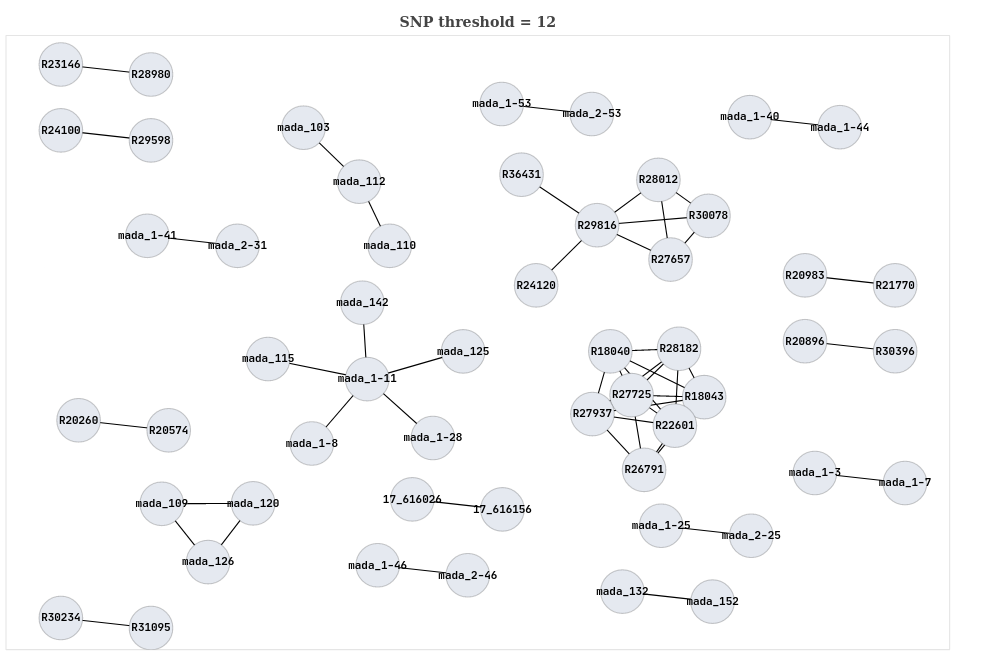
\includegraphics[width=\textwidth]{Appendix1/Figs/compass_clusters_t12.png}
         \caption{}
     \end{subfigure}
        \caption{Transmission clusters from COMPASS SNP calls. Each node represents a sample with edges between samples indicating a SNP distance $\le$ the SNP threshold used for the graph. The SNP thresholds for each graph can be found in the title of each subplot. They are 0, 2, 5, and 12 for \textbf{a}, \textbf{b}, \textbf{c}, and \textbf{d} respectively}
        \label{fig:compass-original-clusters}
\end{figure}

\begin{figure}
     \centering
     \begin{subfigure}[b]{0.45\textwidth}
         \centering
         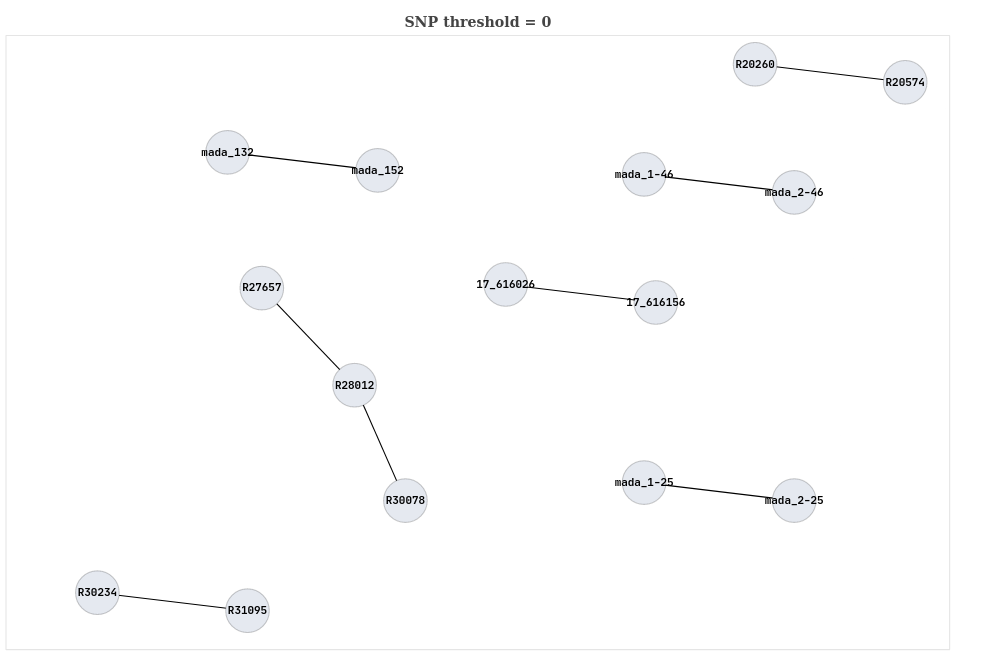
\includegraphics[width=\textwidth]{Appendix1/Figs/bcftools_clusters_t0.png}
         \caption{}
     \end{subfigure}
     \hfill
     \begin{subfigure}[b]{0.45\textwidth}
         \centering
         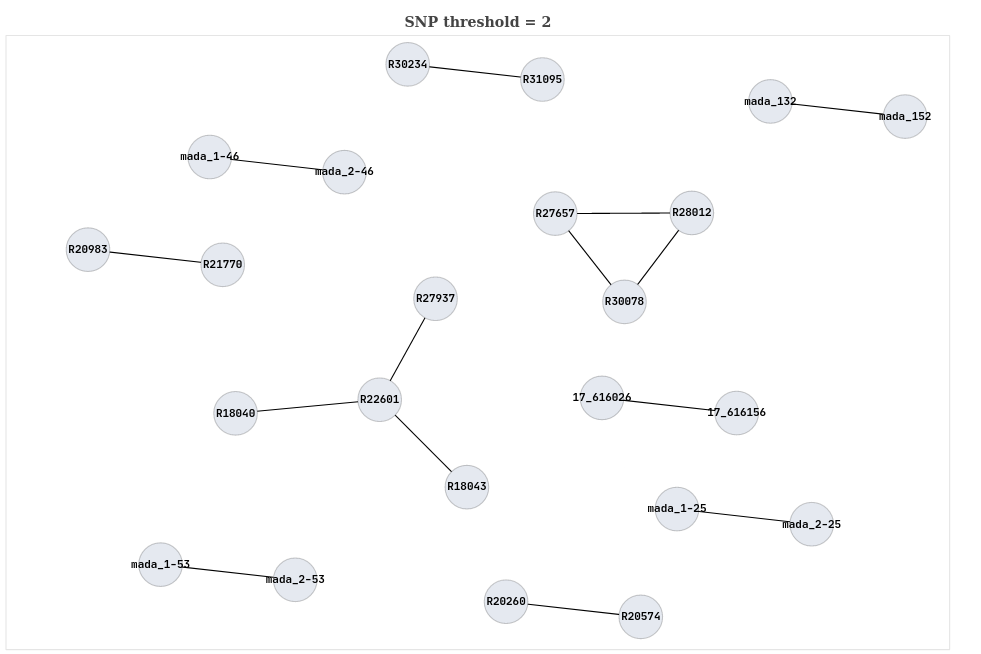
\includegraphics[width=\textwidth]{Appendix1/Figs/bcftools_clusters_t2.png}
         \caption{}
     \end{subfigure}
     \begin{subfigure}[b]{0.45\textwidth}
         \centering
         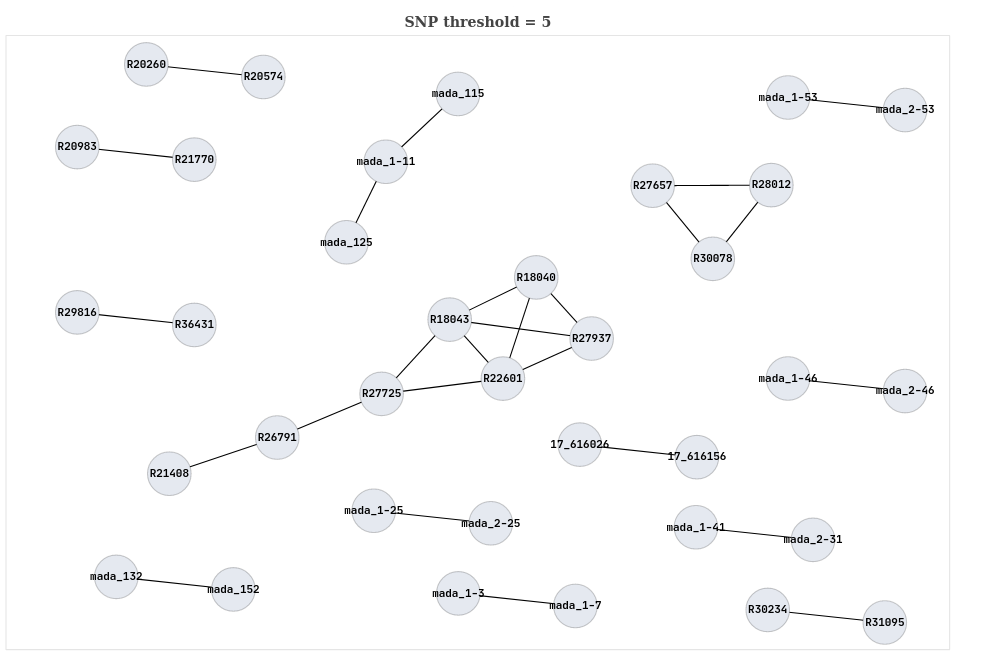
\includegraphics[width=\textwidth]{Appendix1/Figs/bcftools_clusters_t5.png}
         \caption{}
     \end{subfigure}
     \hfill
     \begin{subfigure}[b]{0.45\textwidth}
         \centering
         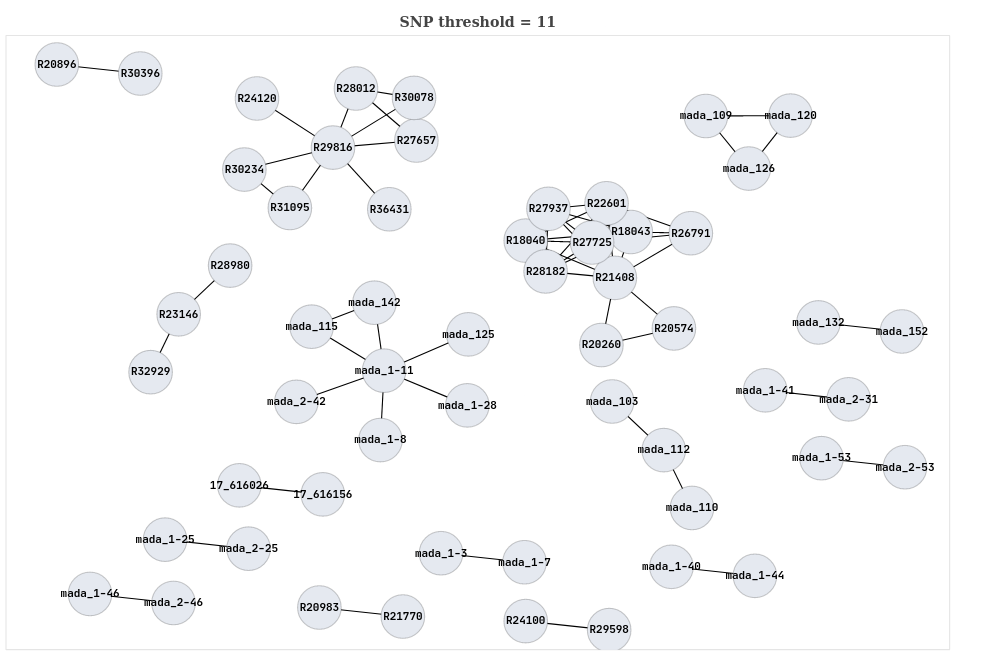
\includegraphics[width=\textwidth]{Appendix1/Figs/bcftools_clusters_t11.png}
         \caption{}
     \end{subfigure}
        \caption{Transmission clusters from \bcftools{} SNP calls. Each node represents a sample with edges between samples indicating a SNP distance $\le$ the SNP threshold used for the graph. The SNP thresholds for each graph can be found in the title of each subplot. They are 0, 2, 5, and 11 for \textbf{a}, \textbf{b}, \textbf{c}, and \textbf{d} respectively}
        \label{fig:bcftools-original-clusters}
\end{figure}

\begin{figure}
     \centering
     \begin{subfigure}[b]{0.45\textwidth}
         \centering
         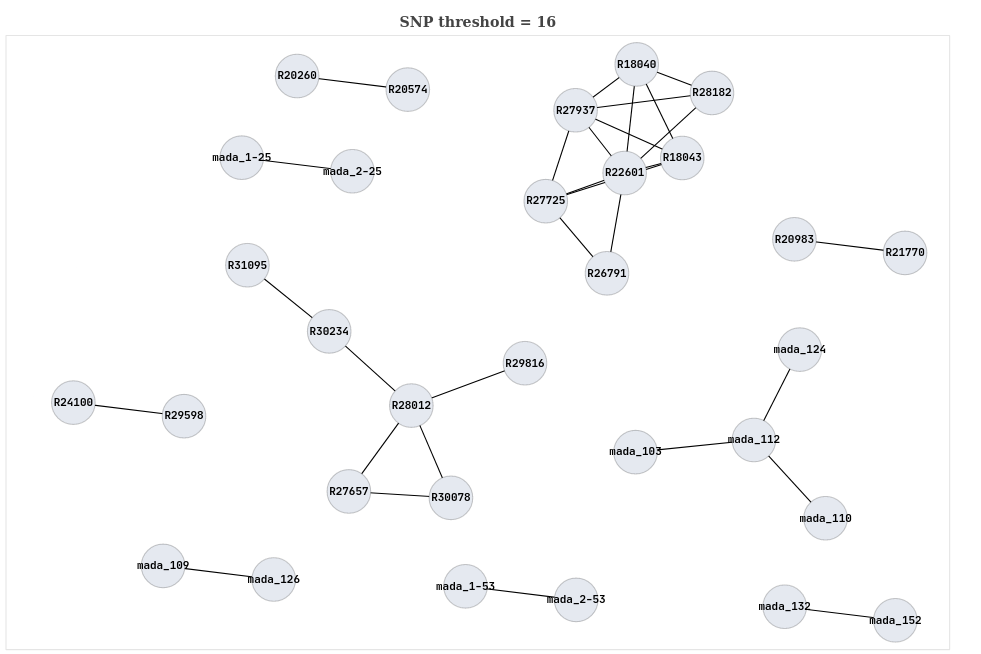
\includegraphics[width=\textwidth]{Appendix1/Figs/map_clusters_t16.png}
         \caption{}
     \end{subfigure}
     \hfill
     \begin{subfigure}[b]{0.45\textwidth}
         \centering
         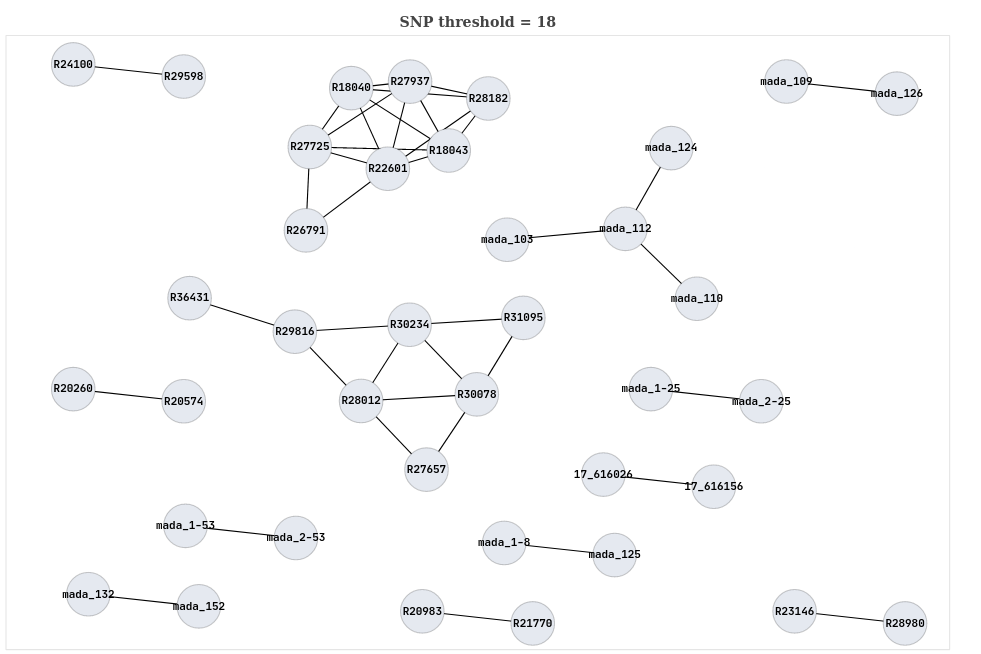
\includegraphics[width=\textwidth]{Appendix1/Figs/map_clusters_t18.png}
         \caption{}
     \end{subfigure}
     \begin{subfigure}[b]{0.45\textwidth}
         \centering
         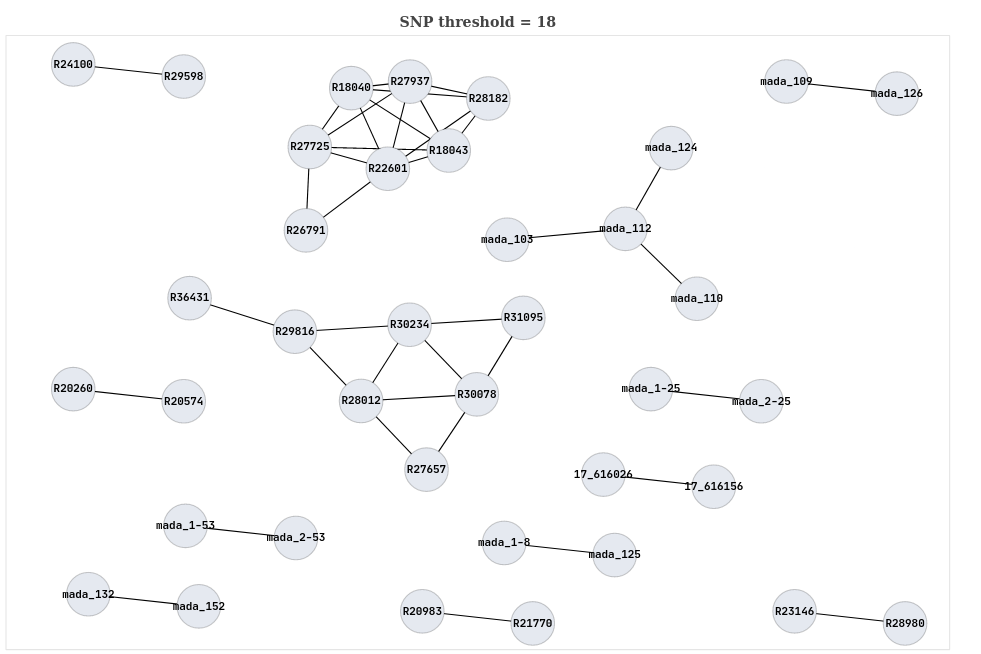
\includegraphics[width=\textwidth]{Appendix1/Figs/map_clusters_t18.png}
         \caption{}
     \end{subfigure}
     \hfill
     \begin{subfigure}[b]{0.45\textwidth}
         \centering
         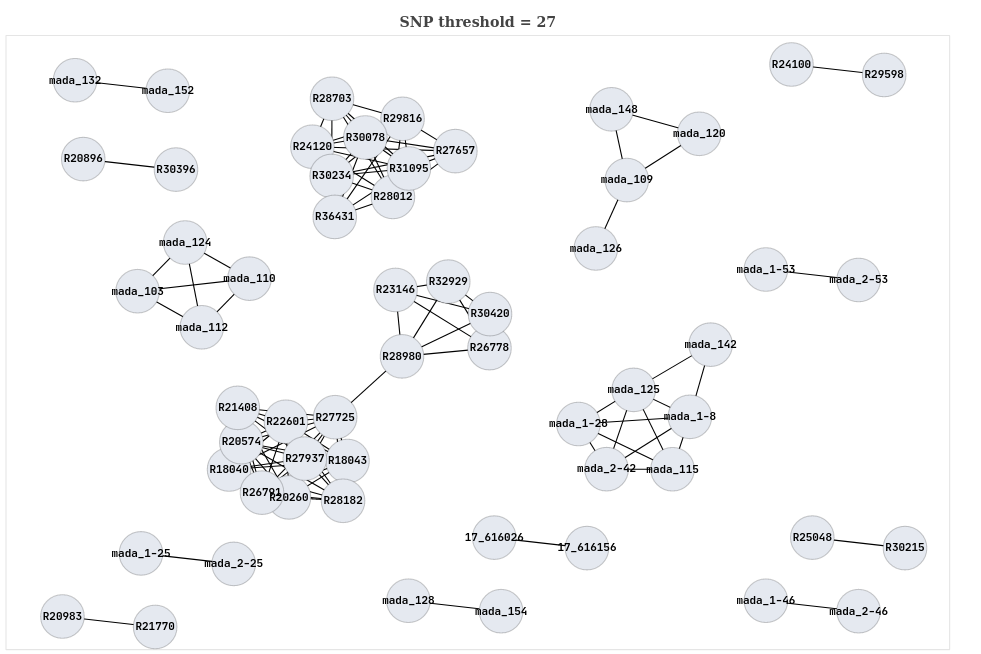
\includegraphics[width=\textwidth]{Appendix1/Figs/map_clusters_t27.png}
         \caption{}
     \end{subfigure}
        \caption{Transmission clusters from \pandora{} single-sample SNP calls. Each node represents a sample with edges between samples indicating a SNP distance $\le$ the SNP threshold used for the graph. The SNP thresholds for each graph can be found in the title of each subplot. They are 16, 18, 18, and 27 for \textbf{a}, \textbf{b}, \textbf{c}, and \textbf{d} respectively}
        \label{fig:map-original-clusters}
\end{figure}

\begin{figure}
     \centering
     \begin{subfigure}[b]{0.45\textwidth}
         \centering
         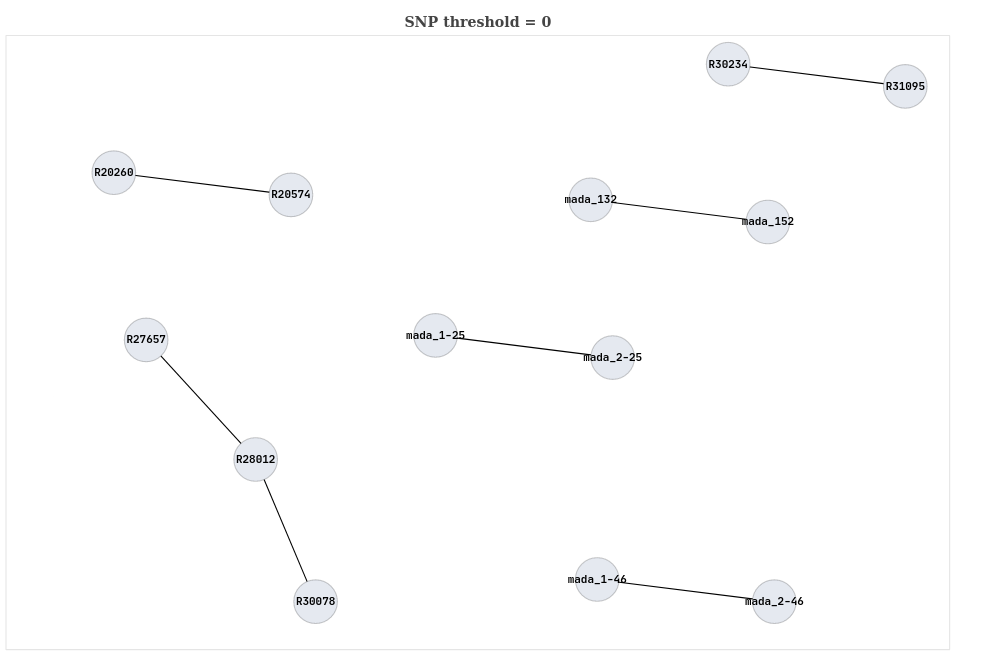
\includegraphics[width=\textwidth]{Appendix1/Figs/compare_clusters_t0.png}
         \caption{}
     \end{subfigure}
     \hfill
     \begin{subfigure}[b]{0.45\textwidth}
         \centering
         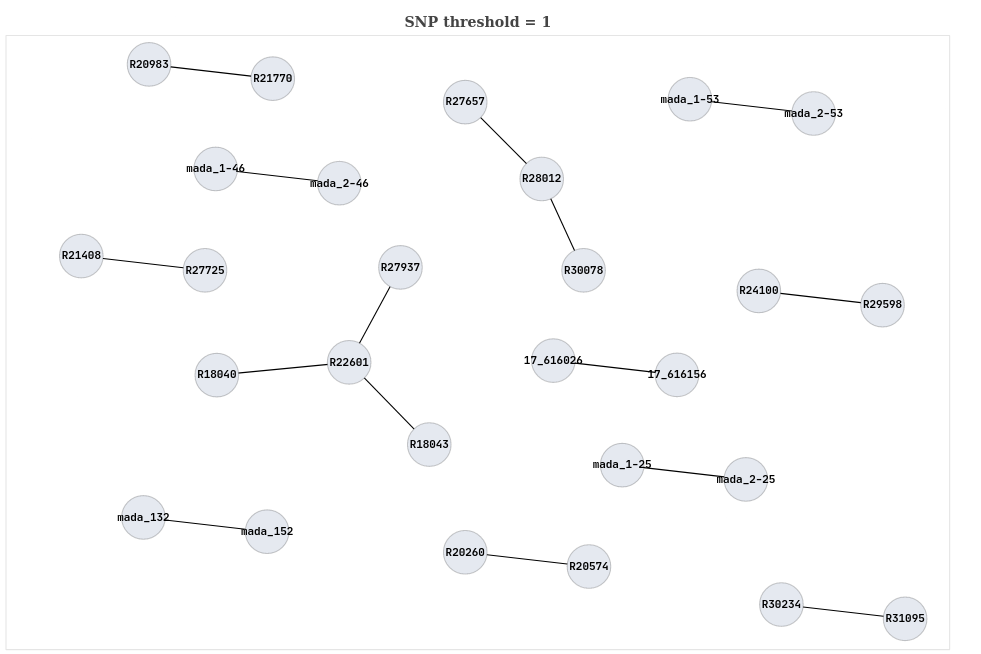
\includegraphics[width=\textwidth]{Appendix1/Figs/compare_clusters_t1.png}
         \caption{}
     \end{subfigure}
     \begin{subfigure}[b]{0.45\textwidth}
         \centering
         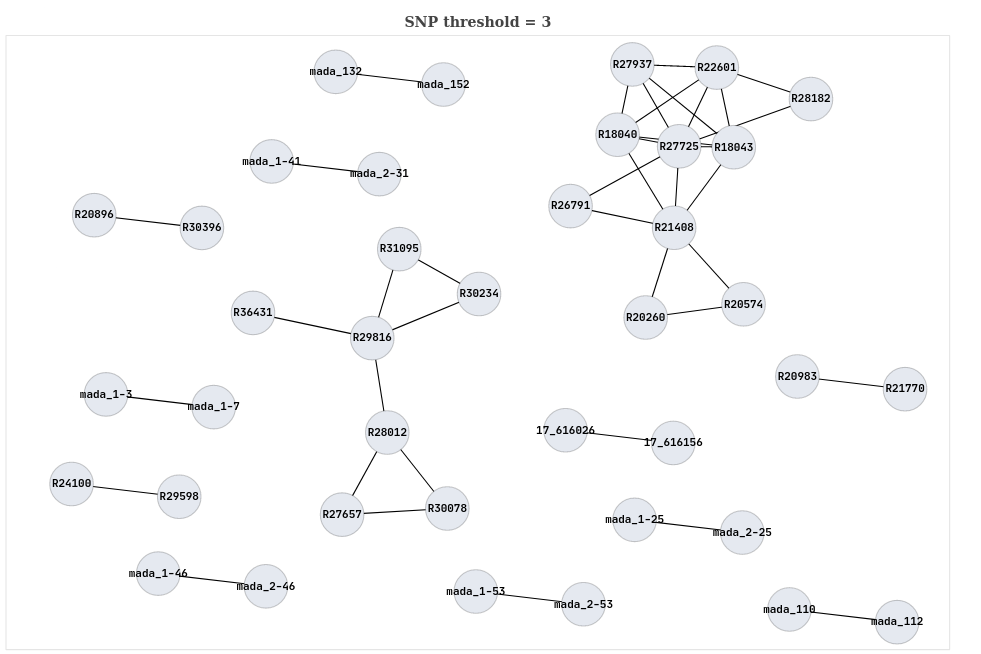
\includegraphics[width=\textwidth]{Appendix1/Figs/compare_clusters_t3.png}
         \caption{}
     \end{subfigure}
     \hfill
     \begin{subfigure}[b]{0.45\textwidth}
         \centering
         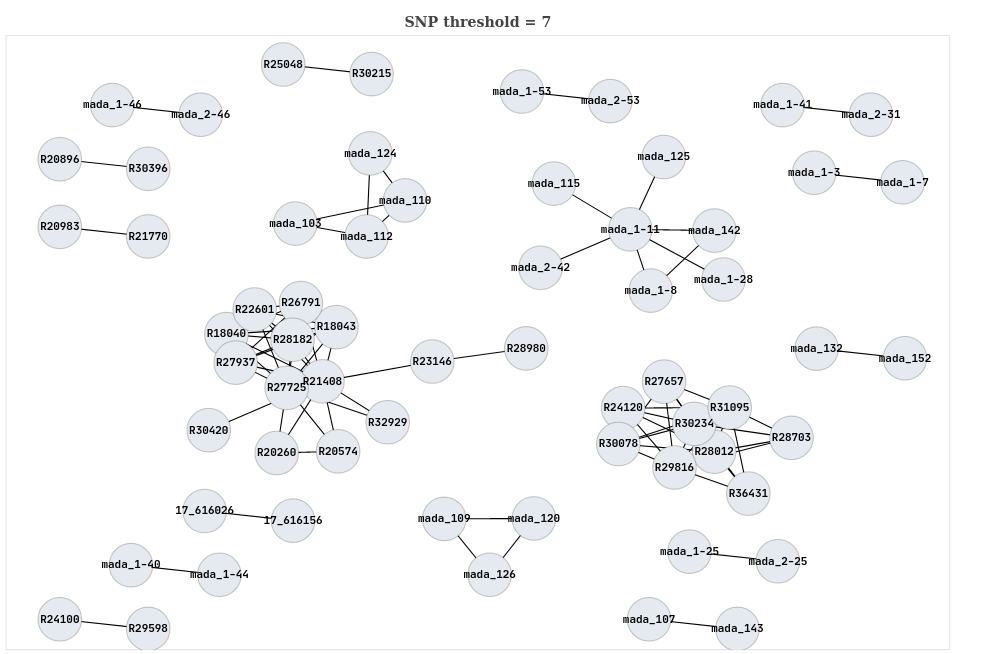
\includegraphics[width=\textwidth]{Appendix1/Figs/compare_clusters_t7.png}
         \caption{}
     \end{subfigure}
        \caption{Transmission clusters from \pandora{} multi-sample SNP calls. Each node represents a sample with edges between samples indicating a SNP distance $\le$ the SNP threshold used for the graph. The SNP thresholds for each graph can be found in the title of each subplot. They are 0, 1, 3, and 7 for \textbf{a}, \textbf{b}, \textbf{c}, and \textbf{d} respectively}
        \label{fig:compare-original-clusters}
\end{figure}

% =====================================
\section{Full mixed technology simulation results}

\begin{longtable}[c]{|l|l|l|l|l|l|l|l|l|l|}
\hline
ratio                   & threshold           & metric & mean  & std   & min   & 25\%  & 50\%  & 75\%  & max   \\ \hline
\endhead
%
\multirow{12}{*}{0.010} & \multirow{3}{*}{0}  & 1-XCR  & 1.000 & 0.001 & 0.985 & 1.000 & 1.000 & 1.000 & 1.000 \\ \cline{3-10} 
                        &                     & SACP   & 0.998 & 0.017 & 0.846 & 1.000 & 1.000 & 1.000 & 1.000 \\ \cline{3-10} 
                        &                     & SACR   & 0.997 & 0.020 & 0.846 & 1.000 & 1.000 & 1.000 & 1.000 \\ \cline{2-10} 
                        & \multirow{3}{*}{2}  & 1-XCR  & 1.000 & 0.000 & 0.992 & 1.000 & 1.000 & 1.000 & 1.000 \\ \cline{3-10} 
                        &                     & SACP   & 1.000 & 0.002 & 0.966 & 1.000 & 1.000 & 1.000 & 1.000 \\ \cline{3-10} 
                        &                     & SACR   & 1.000 & 0.000 & 1.000 & 1.000 & 1.000 & 1.000 & 1.000 \\ \cline{2-10} 
                        & \multirow{3}{*}{5}  & 1-XCR  & 1.000 & 0.002 & 0.984 & 1.000 & 1.000 & 1.000 & 1.000 \\ \cline{3-10} 
                        &                     & SACP   & 0.999 & 0.007 & 0.929 & 1.000 & 1.000 & 1.000 & 1.000 \\ \cline{3-10} 
                        &                     & SACR   & 0.999 & 0.008 & 0.929 & 1.000 & 1.000 & 1.000 & 1.000 \\ \cline{2-10} 
                        & \multirow{3}{*}{12} & 1-XCR  & 1.000 & 0.002 & 0.990 & 1.000 & 1.000 & 1.000 & 1.000 \\ \cline{3-10} 
                        &                     & SACP   & 0.998 & 0.010 & 0.930 & 1.000 & 1.000 & 1.000 & 1.000 \\ \cline{3-10} 
                        &                     & SACR   & 1.000 & 0.002 & 0.965 & 1.000 & 1.000 & 1.000 & 1.000 \\ \hline
\multirow{12}{*}{0.050} & \multirow{3}{*}{0}  & 1-XCR  & 0.999 & 0.003 & 0.985 & 1.000 & 1.000 & 1.000 & 1.000 \\ \cline{3-10} 
                        &                     & SACP   & 0.990 & 0.035 & 0.769 & 1.000 & 1.000 & 1.000 & 1.000 \\ \cline{3-10} 
                        &                     & SACR   & 0.988 & 0.041 & 0.718 & 1.000 & 1.000 & 1.000 & 1.000 \\ \cline{2-10} 
                        & \multirow{3}{*}{2}  & 1-XCR  & 1.000 & 0.002 & 0.992 & 1.000 & 1.000 & 1.000 & 1.000 \\ \cline{3-10} 
                        &                     & SACP   & 0.998 & 0.008 & 0.966 & 1.000 & 1.000 & 1.000 & 1.000 \\ \cline{3-10} 
                        &                     & SACR   & 1.000 & 0.000 & 1.000 & 1.000 & 1.000 & 1.000 & 1.000 \\ \cline{2-10} 
                        & \multirow{3}{*}{5}  & 1-XCR  & 0.997 & 0.006 & 0.967 & 1.000 & 1.000 & 1.000 & 1.000 \\ \cline{3-10} 
                        &                     & SACP   & 0.993 & 0.019 & 0.878 & 1.000 & 1.000 & 1.000 & 1.000 \\ \cline{3-10} 
                        &                     & SACR   & 0.993 & 0.020 & 0.871 & 1.000 & 1.000 & 1.000 & 1.000 \\ \cline{2-10} 
                        & \multirow{3}{*}{12} & 1-XCR  & 0.998 & 0.005 & 0.979 & 1.000 & 1.000 & 1.000 & 1.000 \\ \cline{3-10} 
                        &                     & SACP   & 0.989 & 0.024 & 0.874 & 0.987 & 1.000 & 1.000 & 1.000 \\ \cline{3-10} 
                        &                     & SACR   & 0.998 & 0.007 & 0.965 & 1.000 & 1.000 & 1.000 & 1.000 \\ \hline
\multirow{12}{*}{0.100} & \multirow{3}{*}{0}  & 1-XCR  & 0.999 & 0.004 & 0.985 & 1.000 & 1.000 & 1.000 & 1.000 \\ \cline{3-10} 
                        &                     & SACP   & 0.980 & 0.049 & 0.769 & 1.000 & 1.000 & 1.000 & 1.000 \\ \cline{3-10} 
                        &                     & SACR   & 0.976 & 0.056 & 0.718 & 1.000 & 1.000 & 1.000 & 1.000 \\ \cline{2-10} 
                        & \multirow{3}{*}{2}  & 1-XCR  & 0.999 & 0.002 & 0.992 & 1.000 & 1.000 & 1.000 & 1.000 \\ \cline{3-10} 
                        &                     & SACP   & 0.997 & 0.010 & 0.966 & 1.000 & 1.000 & 1.000 & 1.000 \\ \cline{3-10} 
                        &                     & SACR   & 1.000 & 0.000 & 1.000 & 1.000 & 1.000 & 1.000 & 1.000 \\ \cline{2-10} 
                        & \multirow{3}{*}{5}  & 1-XCR  & 0.994 & 0.009 & 0.959 & 0.984 & 1.000 & 1.000 & 1.000 \\ \cline{3-10} 
                        &                     & SACP   & 0.987 & 0.025 & 0.878 & 0.982 & 1.000 & 1.000 & 1.000 \\ \cline{3-10} 
                        &                     & SACR   & 0.989 & 0.025 & 0.871 & 1.000 & 1.000 & 1.000 & 1.000 \\ \cline{2-10} 
                        & \multirow{3}{*}{12} & 1-XCR  & 0.995 & 0.006 & 0.969 & 0.990 & 1.000 & 1.000 & 1.000 \\ \cline{3-10} 
                        &                     & SACP   & 0.975 & 0.033 & 0.855 & 0.943 & 0.987 & 1.000 & 1.000 \\ \cline{3-10} 
                        &                     & SACR   & 0.997 & 0.010 & 0.965 & 1.000 & 1.000 & 1.000 & 1.000 \\ \hline
\multirow{12}{*}{0.250} & \multirow{3}{*}{0}  & 1-XCR  & 0.996 & 0.006 & 0.985 & 1.000 & 1.000 & 1.000 & 1.000 \\ \cline{3-10} 
                        &                     & SACP   & 0.958 & 0.067 & 0.769 & 0.923 & 1.000 & 1.000 & 1.000 \\ \cline{3-10} 
                        &                     & SACR   & 0.948 & 0.078 & 0.718 & 0.872 & 1.000 & 1.000 & 1.000 \\ \cline{2-10} 
                        & \multirow{3}{*}{2}  & 1-XCR  & 0.998 & 0.003 & 0.992 & 0.992 & 1.000 & 1.000 & 1.000 \\ \cline{3-10} 
                        &                     & SACP   & 0.991 & 0.015 & 0.966 & 0.966 & 1.000 & 1.000 & 1.000 \\ \cline{3-10} 
                        &                     & SACR   & 1.000 & 0.000 & 1.000 & 1.000 & 1.000 & 1.000 & 1.000 \\ \cline{2-10} 
                        & \multirow{3}{*}{5}  & 1-XCR  & 0.985 & 0.013 & 0.943 & 0.975 & 0.984 & 1.000 & 1.000 \\ \cline{3-10} 
                        &                     & SACP   & 0.972 & 0.035 & 0.878 & 0.949 & 0.982 & 1.000 & 1.000 \\ \cline{3-10} 
                        &                     & SACR   & 0.979 & 0.035 & 0.871 & 0.943 & 1.000 & 1.000 & 1.000 \\ \cline{2-10} 
                        & \multirow{3}{*}{12} & 1-XCR  & 0.988 & 0.008 & 0.969 & 0.979 & 0.990 & 0.990 & 1.000 \\ \cline{3-10} 
                        &                     & SACP   & 0.946 & 0.042 & 0.842 & 0.915 & 0.943 & 0.984 & 1.000 \\ \cline{3-10} 
                        &                     & SACR   & 0.994 & 0.013 & 0.965 & 1.000 & 1.000 & 1.000 & 1.000 \\ \hline
\multirow{12}{*}{0.500} & \multirow{3}{*}{0}  & 1-XCR  & 0.993 & 0.007 & 0.985 & 0.985 & 1.000 & 1.000 & 1.000 \\ \cline{3-10} 
                        &                     & SACP   & 0.941 & 0.076 & 0.769 & 0.846 & 1.000 & 1.000 & 1.000 \\ \cline{3-10} 
                        &                     & SACR   & 0.929 & 0.089 & 0.718 & 0.846 & 1.000 & 1.000 & 1.000 \\ \cline{2-10} 
                        & \multirow{3}{*}{2}  & 1-XCR  & 0.996 & 0.004 & 0.992 & 0.992 & 1.000 & 1.000 & 1.000 \\ \cline{3-10} 
                        &                     & SACP   & 0.983 & 0.017 & 0.966 & 0.966 & 1.000 & 1.000 & 1.000 \\ \cline{3-10} 
                        &                     & SACR   & 1.000 & 0.000 & 1.000 & 1.000 & 1.000 & 1.000 & 1.000 \\ \cline{2-10} 
                        & \multirow{3}{*}{5}  & 1-XCR  & 0.971 & 0.015 & 0.943 & 0.959 & 0.967 & 0.984 & 1.000 \\ \cline{3-10} 
                        &                     & SACP   & 0.952 & 0.037 & 0.878 & 0.929 & 0.949 & 0.976 & 1.000 \\ \cline{3-10} 
                        &                     & SACR   & 0.974 & 0.037 & 0.871 & 0.929 & 1.000 & 1.000 & 1.000 \\ \cline{2-10} 
                        & \multirow{3}{*}{12} & 1-XCR  & 0.981 & 0.008 & 0.969 & 0.979 & 0.979 & 0.990 & 1.000 \\ \cline{3-10} 
                        &                     & SACP   & 0.906 & 0.043 & 0.842 & 0.861 & 0.911 & 0.930 & 1.000 \\ \cline{3-10} 
                        &                     & SACR   & 0.991 & 0.015 & 0.965 & 0.965 & 1.000 & 1.000 & 1.000 \\ \hline
\multirow{12}{*}{0.750} & \multirow{3}{*}{0}  & 1-XCR  & 0.989 & 0.006 & 0.985 & 0.985 & 0.985 & 1.000 & 1.000 \\ \cline{3-10} 
                        &                     & SACP   & 0.955 & 0.069 & 0.769 & 0.923 & 1.000 & 1.000 & 1.000 \\ \cline{3-10} 
                        &                     & SACR   & 0.945 & 0.080 & 0.718 & 0.872 & 1.000 & 1.000 & 1.000 \\ \cline{2-10} 
                        & \multirow{3}{*}{2}  & 1-XCR  & 0.994 & 0.003 & 0.992 & 0.992 & 0.992 & 0.992 & 1.000 \\ \cline{3-10} 
                        &                     & SACP   & 0.974 & 0.015 & 0.966 & 0.966 & 0.966 & 0.966 & 1.000 \\ \cline{3-10} 
                        &                     & SACR   & 1.000 & 0.000 & 1.000 & 1.000 & 1.000 & 1.000 & 1.000 \\ \cline{2-10} 
                        & \multirow{3}{*}{5}  & 1-XCR  & 0.958 & 0.014 & 0.943 & 0.943 & 0.959 & 0.967 & 1.000 \\ \cline{3-10} 
                        &                     & SACP   & 0.945 & 0.032 & 0.878 & 0.949 & 0.949 & 0.970 & 1.000 \\ \cline{3-10} 
                        &                     & SACR   & 0.984 & 0.030 & 0.871 & 1.000 & 1.000 & 1.000 & 1.000 \\ \cline{2-10} 
                        & \multirow{3}{*}{12} & 1-XCR  & 0.974 & 0.006 & 0.969 & 0.969 & 0.969 & 0.979 & 0.990 \\ \cline{3-10} 
                        &                     & SACP   & 0.875 & 0.035 & 0.842 & 0.845 & 0.857 & 0.902 & 0.975 \\ \cline{3-10} 
                        &                     & SACR   & 0.994 & 0.013 & 0.965 & 1.000 & 1.000 & 1.000 & 1.000 \\ \hline
\multirow{12}{*}{0.900} & \multirow{3}{*}{0}  & 1-XCR  & 0.987 & 0.004 & 0.985 & 0.985 & 0.985 & 0.985 & 1.000 \\ \cline{3-10} 
                        &                     & SACP   & 0.980 & 0.048 & 0.769 & 1.000 & 1.000 & 1.000 & 1.000 \\ \cline{3-10} 
                        &                     & SACR   & 0.976 & 0.055 & 0.718 & 1.000 & 1.000 & 1.000 & 1.000 \\ \cline{2-10} 
                        & \multirow{3}{*}{2}  & 1-XCR  & 0.993 & 0.002 & 0.992 & 0.992 & 0.992 & 0.992 & 1.000 \\ \cline{3-10} 
                        &                     & SACP   & 0.970 & 0.011 & 0.966 & 0.966 & 0.966 & 0.966 & 1.000 \\ \cline{3-10} 
                        &                     & SACR   & 1.000 & 0.000 & 1.000 & 1.000 & 1.000 & 1.000 & 1.000 \\ \cline{2-10} 
                        & \multirow{3}{*}{5}  & 1-XCR  & 0.948 & 0.009 & 0.943 & 0.943 & 0.943 & 0.951 & 0.984 \\ \cline{3-10} 
                        &                     & SACP   & 0.944 & 0.023 & 0.878 & 0.949 & 0.949 & 0.949 & 1.000 \\ \cline{3-10} 
                        &                     & SACR   & 0.992 & 0.022 & 0.929 & 1.000 & 1.000 & 1.000 & 1.000 \\ \cline{2-10} 
                        & \multirow{3}{*}{12} & 1-XCR  & 0.971 & 0.005 & 0.969 & 0.969 & 0.969 & 0.969 & 0.990 \\ \cline{3-10} 
                        &                     & SACP   & 0.855 & 0.022 & 0.842 & 0.845 & 0.845 & 0.857 & 0.971 \\ \cline{3-10} 
                        &                     & SACR   & 0.997 & 0.010 & 0.965 & 1.000 & 1.000 & 1.000 & 1.000 \\ \hline
\caption{Summary statistics from the simulations of various sequencing technology ratios and the assessment of transmission clusters produced at different SNP thresholds in \autoref{sec:mixed-clustering}. SACR=sample-averaged cluster recall; SACP=sample-average cluster precision; XCR=excess clustering rate; std=standard deviation.}
\label{tab:mixed-sims-full}\\
\end{longtable}